This chapter details the methodological framework designed to investigate and generate counterfactual explanations (CEs) in the context of image based autonomous driving decisions. At the core of this framework is a deep generative model, specifically a variational autoencoder (VAE) trained to encode and reconstruct high-dimensional driving scenes collected from the CARLA simulator. The learned latent space representations are used to train a classifier that predicts discrete driving actions STOP, GO, RIGHT, and LEFT.

To induce counterfactual changes, a range of masking techniques are applied either to the input images or directly within the latent space. These perturbations aim to identify minimal yet semantically meaningful modifications that result in altered classifier predictions. The effectiveness of each method is assessed through both algorithmic metrics (e.g., reconstruction loss, PSNR, and SSIM) and a human evaluation study that captures interpretability, plausibility, and visual coherence from a user’s perspective.

The design and implementation of this framework are structured around four central research questions (RQs), initially introduced in Chapter~\ref{Introduction} and now revisited with a focus on their technical realization. Each RQ targets a distinct component of the system from representation learning and loss function optimization to comparative evaluation of explanation strategies. The implementation strategies are detailed in the sections that follow, with relevant modules cross-referenced (e.g., \cref{sec:vae}, \cref{sec:classifier_architectures}, and \cref{sec:feature_masking_pipeline}) to guide the reader through the complete example-based explainability pipeline.

\vspace{1em}

\textbf{RQ1: VAE and Classifier Implementation} \\
\textit{How can deep generative models be implemented to effectively encode and reconstruct high-dimensional RGB input images of driving scenes for compact and interpretable representation learning in autonomous driving systems?}

To address this research question, the following implementation strategy was adopted.

\vspace{-1em}

\paragraph{Implementation:} A Variational Autoencoder (VAE) is implemented to learn compact and semantically meaningful latent representations from high-dimensional RGB images (\(80 \times 160 \times 3\)) collected from a simulated driving environment. The VAE architecture consists of a deep convolutional encoder-decoder framework trained in an unsupervised manner, minimizing reconstruction loss while regularizing the latent space distribution. Key design considerations include latent dimensionality selection (e.g., 128-dim), KL divergence annealing for stable training, and comparative analysis of reconstruction loss functions (Mean Squared Error vs. Log-Cosh). Although the VAE is trained without using class labels (i.e., in an unsupervised manner), its learned latent representations are later used to train separate classifiers for both binary (e.g., STOP vs. GO) and multi-class (STOP, GO, LEFT, RIGHT) classification tasks. This setup allows us to indirectly assess the quality and semantic structure of the latent space through downstream performance on these classification problems.


The architectural and training details of the VAE are elaborated in \cref{sec:vae}, while classifier models trained on the VAE’s latent space are described in \cref{sec:classifier_architectures}. Evaluation results, reconstruction metrics, and visual analyses are presented in \cref{sec:vae_evaluation} and \cref{sec:classifier_eval}.

\vspace{1em}

\textbf{RQ2: Loss Function Analysis} \\
\textit{How can loss function modifications in Variational Autoencoders (VAEs) optimize image reconstruction quality in autonomous driving tasks?}

\vspace{-1em}

\paragraph{Implementation:} To address RQ2, the VAE introduced in \cref{sec:vae} is trained using two different reconstruction loss functions, Mean Squared Error (MSE) and Log-Cosh. The Log-Cosh loss is selected based on prior work~\cite{chen2019log}, which shows that it balances sensitivity to small deviations (like L2) with robustness to outliers (like L1), making it suitable for visual data.
        
Both losses are integrated into an otherwise identical training setup. KL divergence annealing is consistently applied, and hyperparameters (learning rate, batch size, optimizer) are held constant to ensure fair comparison. The models are trained independently with the same dataset. The implementation of these are explained in the \cref{subsec:vae_loss}, corresponding evaluations and results are discussed in the \cref{subsec:vae_quant_comparison}.


\vspace{1em}

\textbf{RQ3: Comparative Evaluation of Masking Techniques} \\
\textit{How do different masking techniques impact the effectiveness and efficiency of counterfactual explanation generation, in terms of coverage, computational cost, method overlap, and failure rate?}

\vspace{-1em}

\paragraph{Implementation:}To explore RQ3, multiple masking strategies are implemented to generate counterfactual explanations (CEs) based on altering either the input image space or the latent space of a trained VAE. Each method is integrated into a unified Counterfactual explanation pipeline that encodes the image, applies a specific masking technique, reconstructs the image using the VAE, and reclassifies it to determine whether a prediction change has occurred. Thus qualifying as a counterfactual explanations.


The full methodology for each masking technique is detailed in \cref{sec:feature_masking_pipeline}, and experimental results for these techniques are presented in \cref{sec:masking_eval}.

\vspace{1em}

\textbf{RQ4: User Study on Counterfactual Preferences}  \\
\textit{Which counterfactual explanation method is most preferred by users when selecting among generated explanations of the same original image? What factors influence user preference?}

\vspace{-1em}

\paragraph{Implementation:}To answer RQ4, a user study is conducted in which participants are shown original driving scene images alongside counterfactual explanations generated using different masking methods (from RQ3). For each image, participants are asked to select the explanation they find most helpful or intuitive and rate it based on three key dimensions:

\begin{itemize}
    \item \textbf{Interpretability:} How easily can the user understand why the prediction changed?
    \item \textbf{Plausibility:} Does the counterfactual look like a realistic driving scene?
    \item \textbf{Visual Coherence:} Is the reconstruction smooth, artifact-free, and consistent with the original image?
\end{itemize}

Details of the user study design and AI evaluation pipeline along with comparative results are discussed in \cref{sec:human_evaluation}.

\section{Experimental Setup}

All experiments in this thesis were conducted in a Linux environment to ensure compatibility with the CARLA simulator and associated tools. The setup was built using \textbf{CARLA version 0.9.15}, an open-source urban driving simulator widely adopted for autonomous driving research. This version provides a flexible and high-fidelity simulation environment, making it suitable for collecting diverse, labeled driving data under various rural and urban conditions.

To maintain compatibility with CARLA’s Python API, \textbf{Python version 3.7} was used for dataset collection. This version is recommended by CARLA’s developers to avoid API and dependency conflicts. The dataset was collected using two CARLA maps \textbf{Town03} and \textbf{Town07}~\cite{CARLA2024}, provide varied driving topologies as shown in Figure~\ref{fig:carla_maps}. These maps were chosen due to their varied road layouts and environmental features, which provide rich scenarios for evaluating counterfactual explanations. Example simulation scenes demonstrating diverse driving and weather conditions are presented in Figure~\ref{fig:carla_scenes}. Users replicating this setup should download the CARLA server (v0.9.15) along with the additional maps from the \textit{official CARLA repository}~\cite{CARLA2024docs}. Once downloaded, the maps must be copied into the main CARLA directory to ensure proper integration.

\begin{figure}[htbp]
    \centering
    \begin{subfigure}{0.48\textwidth}
        \centering
        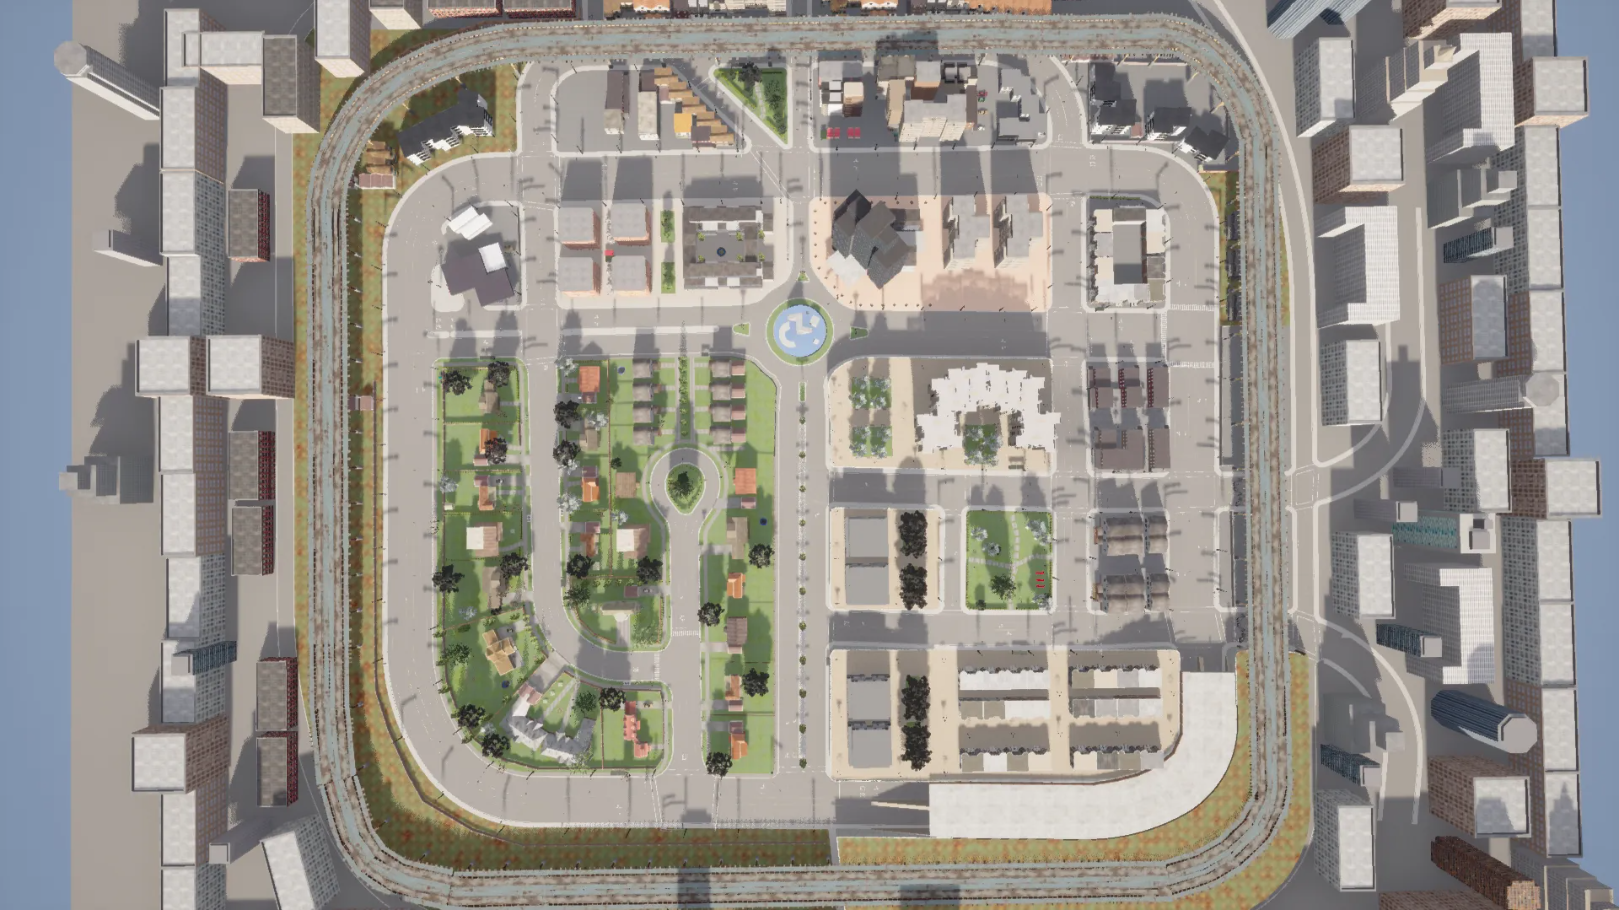
\includegraphics[width=\linewidth]{img/carla/town03.png}
        \caption{CARLA Town03 layout}
    \end{subfigure}
    \hfill
    \begin{subfigure}{0.48\textwidth}
        \centering
        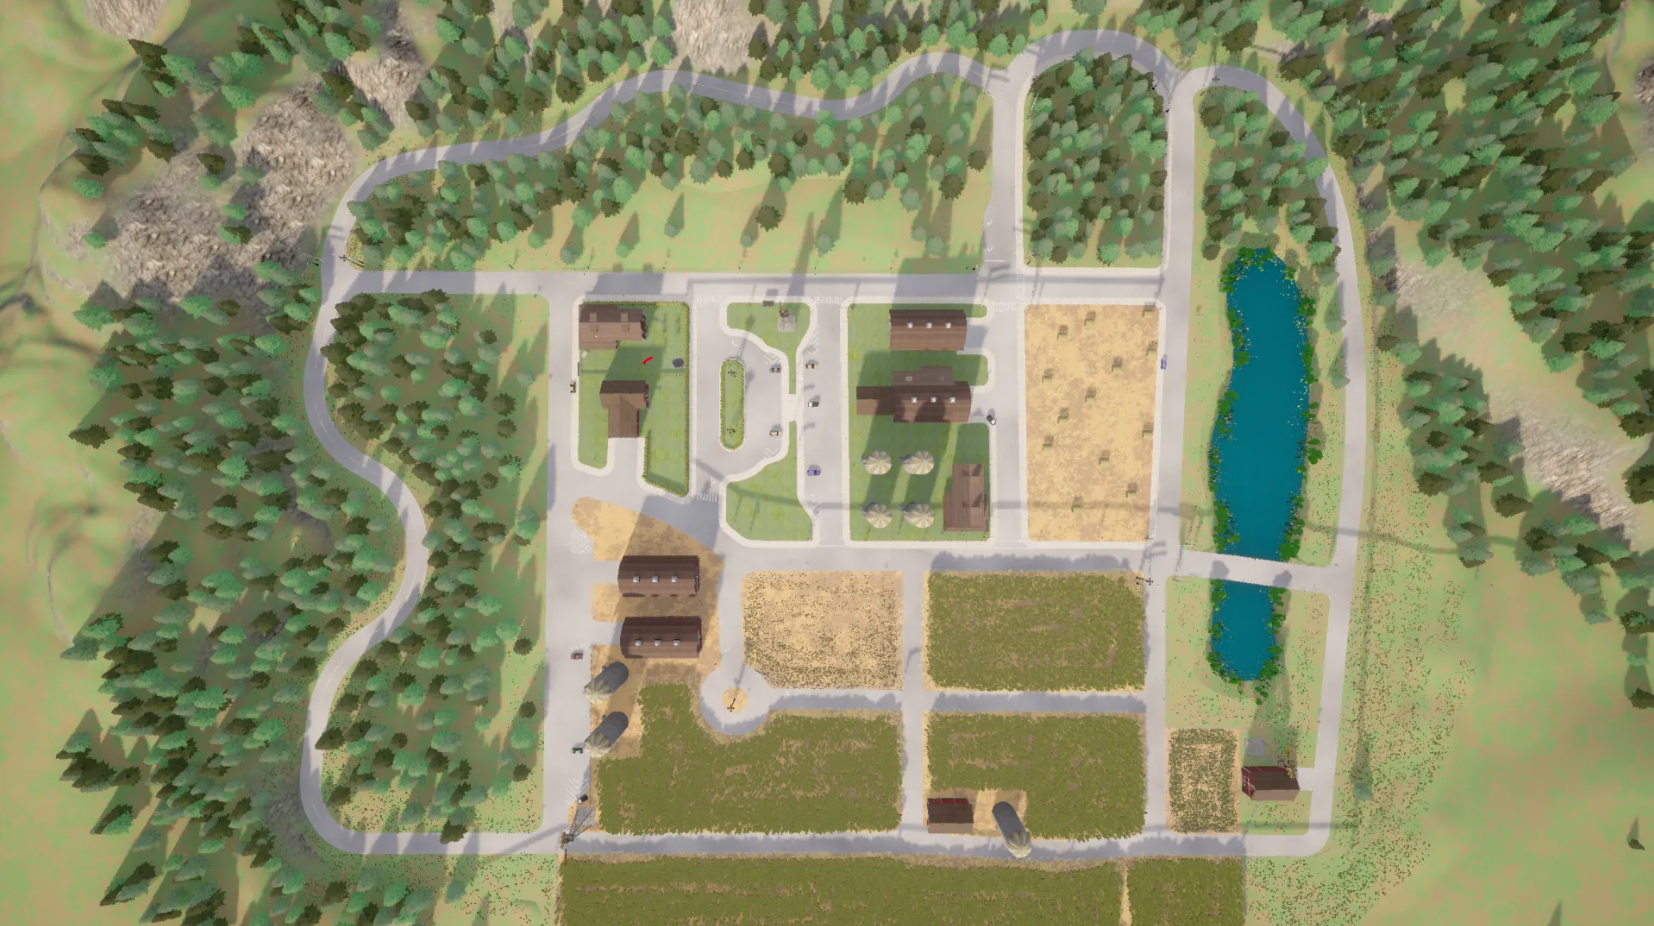
\includegraphics[width=\linewidth]{img/carla/town_7.png}
        \caption{CARLA Town07 layout}
    \end{subfigure}
    \caption{Top-down map layouts of the selected CARLA towns used for dataset collection~\cite{CARLA2024}}.
    \label{fig:carla_maps}
\end{figure}

\begin{figure}[h]
    \centering
    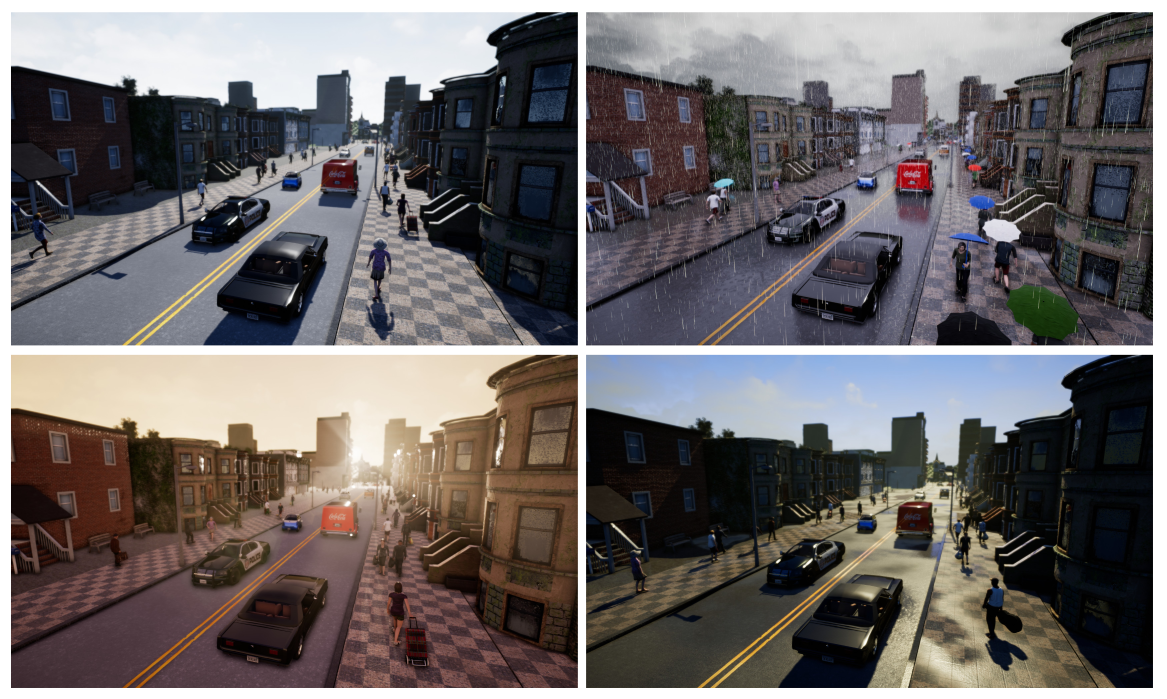
\includegraphics[width=0.9\linewidth]{img/carla/CARLA_Environment.png}
    \caption[CARLA scenes under diverse conditions]{3D Sample scenes from CARLA showcasing diverse conditions. The images illustrate a variety of urban and rural settings, with diverse lighting and weather conditions, including sunny, foggy, rainy, and snowy scenarios. Each scene highlights the flexibility of CARLA in simulating realistic driving environments for autonomous vehicle testing.}
    \label{fig:carla_scenes}
\end{figure}



Before executing any client-side scripts for dataset collection, it is essential to start the CARLA server using the following command in the CARLA root directory: ./CarlaUE4.sh


This launches the CARLA simulation in the Unreal Engine environment. For smooth operation, it is recommended to run the project on a system with at least \textbf{16 GB of RAM}, a dedicated GPU (e.g., \textbf{NVIDIA RTX series}), and \textbf{Ubuntu 18.04 or 20.04 LTS}. 

For the development and training of the Variational Autoencoder (VAE) and classifier models, we used \textbf{Python version 3.11 or higher}. This was necessary to avoid compatibility issues with newer versions of PyTorch, which are not well supported on older Python versions like 3.7. While dataset collection was handled using Python 3.7, the core machine learning model development required a more modern Python environment.  

To monitor and interpret various aspects of model training such as loss, accuracy, weight distributions, and layer activations we used \textbf{TensorBoard}. It provided valuable insights into training behavior and helped fine-tune model performance.

\section{Dataset Collection, Labeling, and Splitting Process}

To train and evaluate the proposed models effectively, a high-quality and well-structured dataset was essential. A systematic data preparation pipeline consisting of three key stages \textit{collection}, \textit{labeling}, and \textit{splitting}. The dataset was first collected using the CARLA simulator, which offers a controllable and realistic environment for simulating diverse driving scenarios. Following data collection, a precise rule-based labeling strategy was applied using vehicle control signals to assign meaningful class labels. Finally, the labeled dataset was partitioned into training and testing subsets to ensure class balance and prevent data leakage. This structured pipeline ensured consistency, and reproducibility  throughout the experimental workflow.

\subsection{Dataset Collection}

The dataset was collected using the CARLA simulator~\cite{CARLA2024docs}. An Audi A2 vehicle was deployed in autopilot mode to autonomously navigate the environment while capturing RGB images and corresponding control signals. A front mounted RGB camera was configured with a 125° field of view (FoV) and a resolution of $160 \times 80$ pixels. This resolution was selected to balance computational efficiency with sufficient visual detail for model learning.

A total of approximately 12,000 images were collected under varied driving scenarios. Each image was paired with the vehicle’s control parameters steering, throttle, and brake. The \textit{steering angle} ranged from $-1$ (full left) to $1$ (full right), while \textit{throttle} and \textit{brake} values ranged from $0$ to $1$, representing the intensity of acceleration and braking, respectively. This multi-modal data captured both visual context and driving behavior. The resulting dataset served as the foundation for both binary (STOP vs. GO) and multi-class (STOP, GO, LEFT, RIGHT) classification tasks.

The \textit{steering angle} ranged from $-1$ (full left) to $1$ (full right), while \textit{throttle} and \textit{brake} values ranged from $0$ to $1$, representing the intensity of acceleration and braking, respectively. Although the full steering range spans ±1, directional labels (LEFT, RIGHT, GO) were based on empirically selected thresholds of ±0.1 to distinguish meaningful turns from straight driving.

\subsection{Dataset Labeling}

The collected data was labeled using a deterministic rule-based strategy derived from the vehicle’s control inputs. Two distinct labeling schemes were implemented to support binary and multi-class classification objectives.

For the \textbf{binary-class scheme}, each frame was labeled as either \texttt{STOP} or \texttt{GO}. A frame was labeled as \texttt{STOP} if the brake value exceeded 0.5 and throttle was less than 0.2. Otherwise, it was labeled as \texttt{GO}. This distinction effectively captured the vehicle's motion state based on braking behavior.

For the \textbf{multi-class scheme}, labels were assigned based on prioritized control logic:
\begin{itemize}
    \item \texttt{STOP}, if brake $> 0.5$ and throttle $< 0.2$
    \item \texttt{RIGHT}, if steering $> 0.1$ and brake $< 0.5$
    \item \texttt{LEFT}, if steering $< -0.1$ and brake $< 0.5$
    \item \texttt{GO}, if throttle $> 0.5$ and $|\text{steering}| < 0.1$
\end{itemize}


These thresholds were empirically determined based on the distribution of control signals in the dataset (see \cref{appendix:labeling}, Table~\ref{tab:label-thresholds} and Figure~\ref{fig:threshold-histograms}). The labeling logic ensured that each image received a mutually exclusive and semantically meaningful label. The labeling process was fully automated, ensuring reproducibility and eliminating manual bias.

After labeling, the dataset showed natural class imbalance, with STOP and GO dominating and LEFT and RIGHT being underrepresented. To mitigate this, targeted data augmentation was applied to the LEFT and RIGHT classes. Augmentation techniques included horizontal flipping, brightness and contrast adjustment, and slight rotation, preserving semantic integrity while increasing data diversity. Augmented samples retained their original labels, enabling class balancing without compromising label consistency.


\subsection{Dataset Splitting}

Following labeling, the dataset was divided into separate training and testing subsets. The splitting was performed \textit{after} labeling to maintain label integrity and avoid any form of data leakage. Care was taken to ensure that the distribution of class labels remained balanced across both sets. This was critical for promoting fair learning and evaluation, particularly in the multi-class scenario.

The labeled dataset was partitioned using an 80/20 split ratio, where 80\% of the data was used for training and 20\% for testing. This ensured sufficient data for model learning while preserving a representative set for evaluation.

\begin{figure}
    \centering
    \begin{subfigure}{0.48\textwidth}
        \centering
        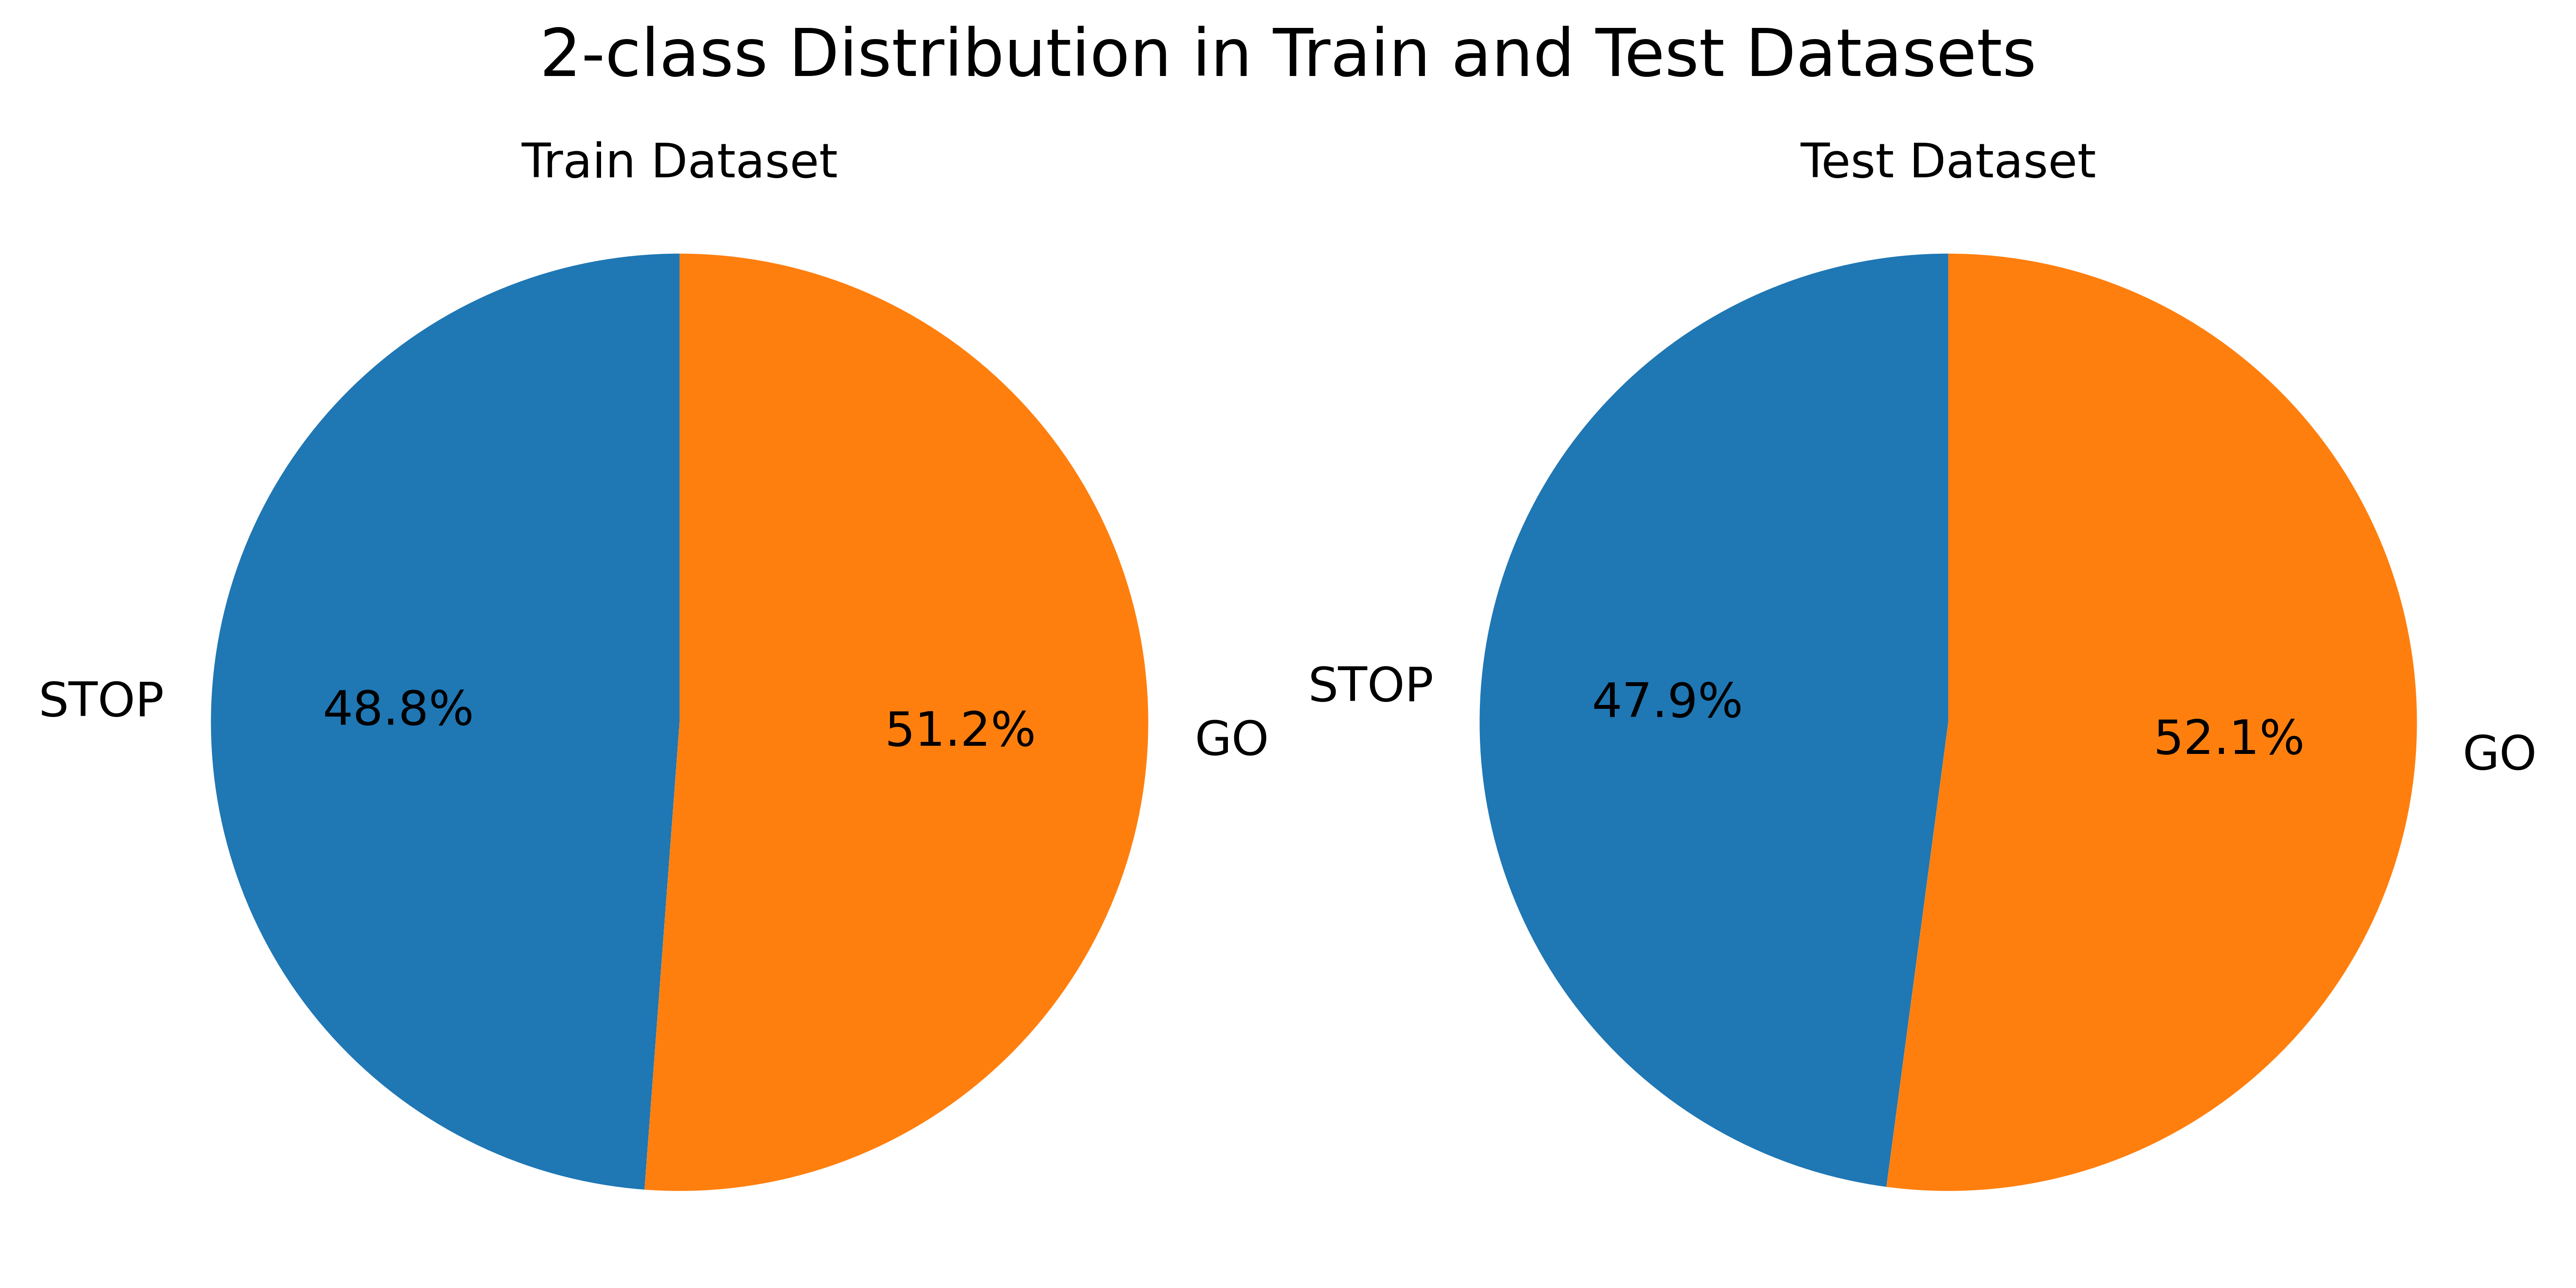
\includegraphics[width=\linewidth]{img/dataset/2-class_distribution_pie_chart.png}
        \caption{Binary class label distribution}
        \label{fig:binary_class_distribution}
    \end{subfigure}
    \hfill
    \begin{subfigure}{0.5\textwidth}
        \centering
        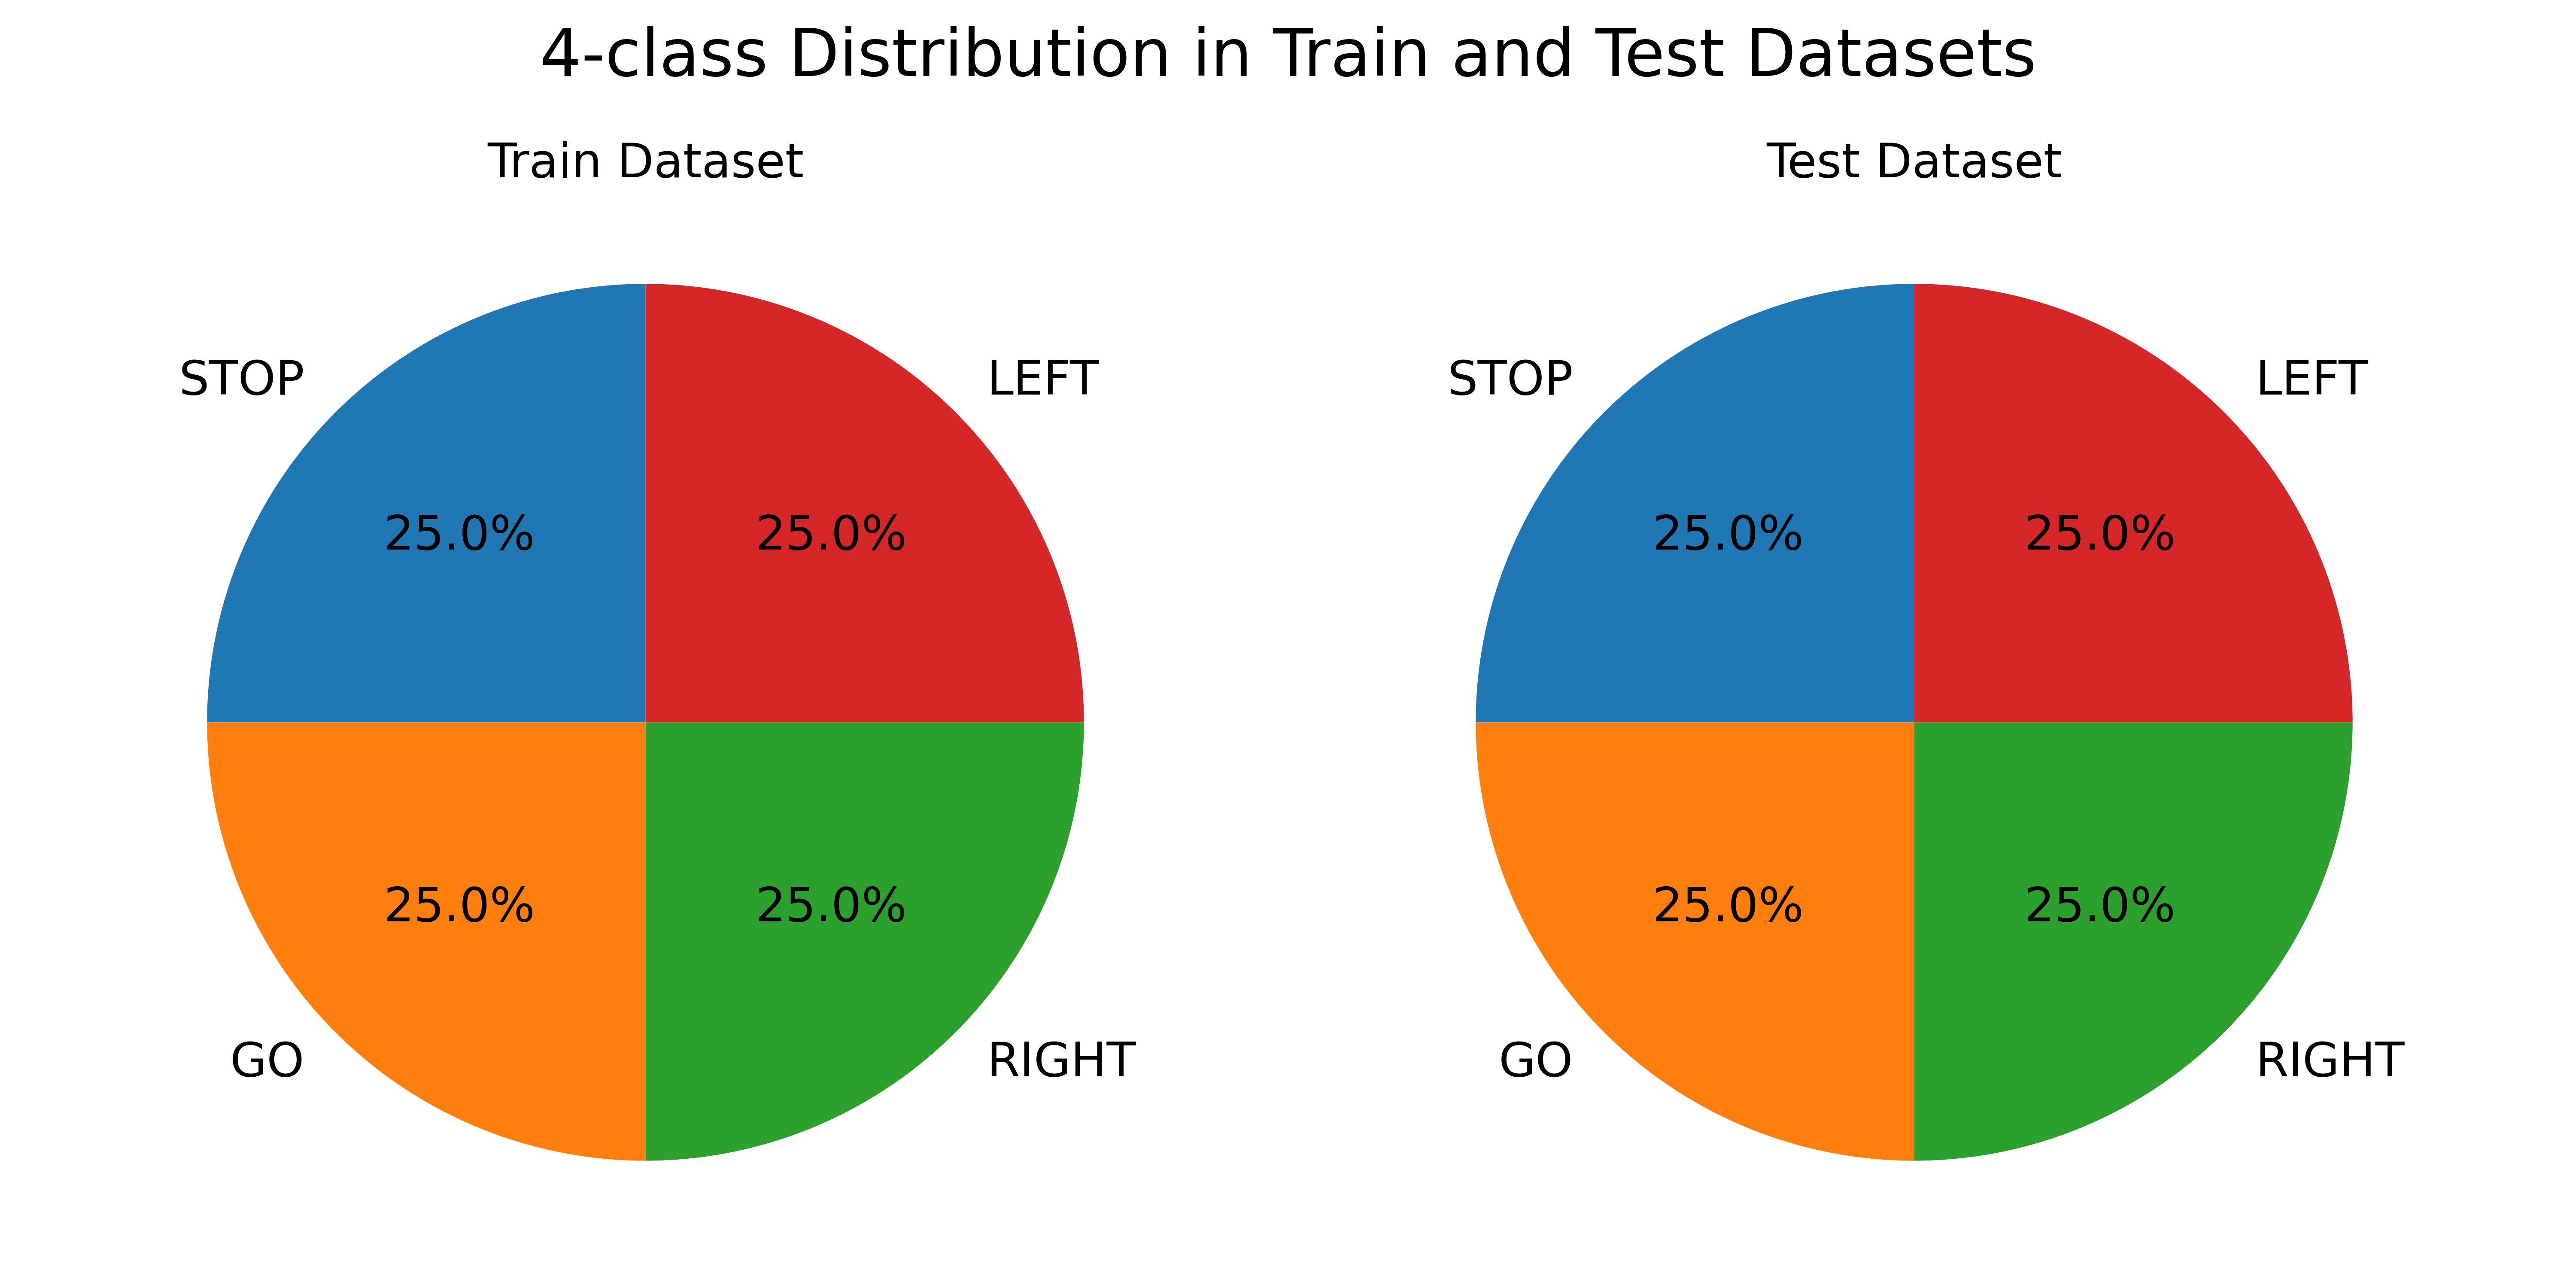
\includegraphics[width=\linewidth]{img/dataset/4-class_distribution_pie_chart.png}
        \caption{multi-class label distribution}
        \label{fig:class_distribution_pie}
    \end{subfigure}
    \caption{Label distributions across training and testing datasets for binary and multi-class classification schemes.}
    \label{fig:label_distribution_combined}
\end{figure}

For the binary classification scheme, the training set contained 4,959 GO and 4,728 STOP samples, while the test set included 1,262 GO and 1,160 STOP samples, maintaining a near-balanced distribution across classes. In the multi-class configuration, STOP and GO had naturally higher counts (3,772 and 3,422 respectively), while LEFT and RIGHT were augmented to match these counts, ensuring class balance. Each class in the final balanced 4-class training set had approximately 3,772 samples, and the corresponding test set contained 926 STOP, 883 GO, 141 LEFT, and 117 RIGHT samples prior to augmentation. The distributions for both schemes are visualized side by side in Figure~\ref{fig:label_distribution_combined}.







\section{Variational Autoencoder (VAE)} \label{sec:vae}

This section outlines the architectural design, training process for the Variational Autoencoder (VAE) used in this work which strongly answers RQ1. The VAE serves as a generative backbone for producing realistic and plausible counterfactual explanations in the context of autonomous driving. Each component of the system is described in detail, along with the rationale for the chosen configurations and metrics.

To generate semantically coherent and visually realistic counterfactual explanations that remain on the data manifold, we adopt a Variational Autoencoder (VAE) as the generative backbone of the system. This approach draws conceptual motivation from the Contrastive Explanation Method (CEM)~\cite{DBLP:journals/corr/abs-1802-07623}, which leverages autoencoders to constrain generated samples within the support of the data distribution. While CEM was originally evaluated on low-dimensional datasets such as MNIST, the application domain involves high-resolution RGB images from complex driving scenarios. Consequently, the VAE architecture, training objective, and optimization strategy were carefully adapted and refined over multiple design iterations.

Meanwhile, Figure~\ref{fig:image_reconstruction_from_vae} shows the image transformation that takes place after it has been fed into the VAE. 

\subsection{VAE Architecture} \label{sec:vae_architecture}

The VAE consists of two primary components, a convolutional encoder that transforms the input image into a latent distribution, and a decoder that reconstructs the image from a sampled latent vector. The encoder and decoder are trained jointly using a variational loss function that enforces both reconstruction fidelity and latent space regularization.

\begin{figure}
    \centering
    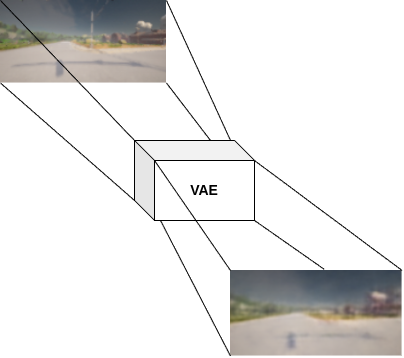
\includegraphics[width=0.5\linewidth]{img/vae/image_reconstructed_from_vae.drawio.png}
    \caption{Image reconstruction from our VAE model}
    \label{fig:image_reconstruction_from_vae}
\end{figure}

\subsubsection{Encoder Architecture} \label{subsubsec:vae_encoder}

The encoder takes an input image of shape $3 \times 80 \times 160$ (RGB, height $\times$ width) and compresses it into a 128-dimensional latent space. The architecture is composed of four convolutional blocks followed by fully connected layers:

\begin{itemize}
    \item \textbf{Conv Layer 1:} 64 filters, kernel size $4 \times 4$, stride 2, no padding. Followed by LeakyReLU.
    \item \textbf{Conv Layer 2:} 128 filters, kernel size $3 \times 3$, stride 2, padding 1. Followed by BatchNorm and LeakyReLU.
    \item \textbf{Conv Layer 3:} 256 filters, kernel size $4 \times 4$, stride 2. Followed by LeakyReLU.
    \item \textbf{Conv Layer 4:} 512 filters, kernel size $3 \times 3$, stride 2. Followed by BatchNorm and LeakyReLU.
\end{itemize}

The final feature map output is flattened and passed through a fully connected layer with 1024 units (with LeakyReLU activation). From this, two separate linear layers output the mean vector $\mu \in \mathbb{R}^{128}$ and log-variance vector $\log\sigma^2 \in \mathbb{R}^{128}$, representing the parameters of the approximate posterior $q(z|x)$.

\subsubsection{Latent Sampling via Reparameterization Trick}
The latent vector $z$ is sampled using the reparameterization trick:
\begin{equation}
z = \mu + \sigma \cdot \epsilon, \quad \epsilon \sim \mathcal{N}(0, I)
\end{equation}
This allows gradient-based optimization through the stochastic sampling process, maintaining end-to-end differentiability. The encoder uses PyTorch’s native implementation of a normal distribution to sample $\epsilon$, and places the distribution tensors on the correct device (CPU or GPU).




\subsubsection{Decoder Architecture} \label{subsubsec:vae_decoder}

The decoder reverses the encoding process and reconstructs an image from the latent vector $z \in \mathbb{R}^{128}$. It consists of two fully connected layers followed by four transposed convolutional layers:

\begin{itemize}
    \item \textbf{Dense Layer 1:} Linear projection from 128 to 1024 units with LeakyReLU.
    \item \textbf{Dense Layer 2:} Linear projection from 1024 to $512 \times 4 \times 9 = 18432$ units, reshaped to $(512, 4, 9)$.
\end{itemize}

The reshaped feature map is then passed through:

\begin{itemize}
    \item \textbf{Deconv Layer 1:} 256 filters, kernel size $4 \times 4$, stride 2, padding 1, output padding (0,1). Followed by LeakyReLU.
    \item \textbf{Deconv Layer 2:} 128 filters, kernel size $4 \times 4$, stride 2, padding 1, output padding (1,1). Followed by LeakyReLU.
    \item \textbf{Deconv Layer 3:} 64 filters, kernel size $4 \times 4$, stride 2. Followed by LeakyReLU.
    \item \textbf{Deconv Layer 4:} 3 filters (RGB), kernel size $4 \times 4$, stride 2. Followed by Sigmoid activation.
\end{itemize}

The final output has shape $3 \times 80 \times 160$, matching the input dimensions. The Sigmoid activation ensures output values lie in the normalized $[0,1]$ range.


\subsection{Image Preprocessing and Augmentation Strategy} \label{subsec:vae_preprocessing}

To improve the generalization ability of the VAE and ensure robustness during training, a set of preprocessing and data augmentation techniques were applied. These techniques were chosen to address common challenges in real-world visual data such as occlusion, viewpoint variation, and overfitting.


During training, the following transformations were applied:
\begin{itemize}
    \item \textbf{Image Resizing:} All images were resized to a fixed resolution of $80 \times 160$ pixels to match the input dimensions required by the encoder.
    \item \textbf{Random Horizontal Flip:} Each image was horizontally flipped with a 50\% probability to simulate mirrored driving conditions and improve generalization.
    % \item \textbf{Random Masking:} A random rectangular region covering 10\% of the image area was masked (set to zero). This augmentation was not only intended to encourage the model to learn robust feature representations by reconstructing occluded regions, but also to strategically expose the VAE to incomplete visual inputs during training. The primary motivation was to ensure that the model remains effective when applied in later stages of this thesis, particularly in masking-based counterfactual generation—where masked or altered inputs are a core component of the explanation process. Training the VAE under such conditions improves its ability to reconstruct high-fidelity outputs even when parts of the input are missing or corrupted.
    \item \textbf{Tensor Conversion:} Images were converted to PyTorch tensors and scaled from [0, 255] to [0.0, 1.0] before being passed to the network.
\end{itemize}


For the testing phase, only the essential deterministic transformations were applied:
\begin{itemize}
    \item Image resizing to $80 \times 160$ pixels
    \item Tensor conversion with pixel scaling
\end{itemize}

\subsection{Hyperparameter Configuration} \label{subsec:hyperparameter_config}
Table~\ref{tab:vae_hyperparams} lists the core hyperparameters used across all VAE training experiments.

\begin{table}[h]
    \centering
    \caption{Hyperparameter settings for VAE training.}
    \label{tab:vae_hyperparams}
    \begin{tabular}{|l|c|}
        \hline
        \textbf{Parameter} & \textbf{Value} \\
        \hline
        Latent Dimension & 128 \\
        Batch Size & 128 \\
        Epochs & 200 \\
        Learning Rate & $1 \times 10^{-4}$ \\
        KL Weight Initial & $5 \times 10^{-5}$ \\
        KL Annealing Schedule & Linear \\
        Optimizer & Adam \\
        Reconstruction Loss & MSE / Log-Cosh (as per experiment) \\
        \hline
    \end{tabular}
\end{table}

\subsection{Training Objective and Optimization Strategy} \label{subsec:vae_loss}

This section presents the training objective and optimization strategy employed to train the Variational Autoencoder (VAE). Including these details in the methodology is essential not only for ensuring reproducibility but also for highlighting the specific design choices that enabled the VAE to learn robust latent representations—central to generating counterfactual explanations in subsequent stages of this work.

The VAE is trained using a composite variational loss function, defined as:
\[
\mathcal{L}_{\text{VAE}} = \mathcal{L}_{\text{recon}} + \lambda_{\text{KL}} \cdot \mathcal{L}_{\text{KL}}
\]
where $\mathcal{L}_{\text{recon}}$ denotes the reconstruction loss, and $\mathcal{L}_{\text{KL}}$ represents the Kullback-Leibler (KL) divergence. The scalar $\lambda_{\text{KL}}$ controls the regularization strength applied to the latent space.

\subsubsection{Reconstruction Loss:} \label{reconstruction_loss}

To assess the impact of different loss formulations on reconstruction quality, two reconstruction loss functions were implemented and compared:
\begin{itemize}
    \item \textbf{Mean Squared Error (MSE):} Measures the average squared difference between corresponding pixel intensities of the input and reconstructed images. It emphasizes pixel-level fidelity and is a standard choice in image reconstruction tasks.
    \item \textbf{log hyperbolic cosine (log-cosh) loss:} A smooth approximation of the Mean Absolute Error (MAE), which behaves like MSE for small differences and like MAE for large ones. It is more tolerant to outliers and encourages sharper reconstructions.
\end{itemize}

Empirical results showed that Log-Cosh yielded smoother and more visually coherent reconstructions during early training epochs, particularly in complex scenes. This finding is supported by prior work, such as Chen et al.~\cite{chen2019log}, and a detailed comparison is presented in \cref{subsec:vae_quant_comparison}.

\paragraph{KL Divergence Regularization:}

The KL divergence term ensures that the learned posterior distribution $q(z|x)$ remains close to the unit Gaussian prior $p(z) = \mathcal{N}(0, I)$:
\begin{equation}
    \mathcal{L}_{\text{KL}} = -\frac{1}{2} \sum_{i=1}^{d} \left(1 + \log\sigma_i^2 - \mu_i^2 - \sigma_i^2\right)
\end{equation}

This regularization promotes a structured latent space, enabling smooth interpolation and semantically meaningful sampling—both of which are essential for generating plausible and interpretable counterfactual explanations. The behaviors qualitative latent space is plotted and explained in \cref{subsubsec:vae_latent_space}.

\paragraph{KL Weight Annealing:}

To prevent the KL term from dominating the loss function prematurely—before the reconstruction objective is sufficiently optimized—a linear annealing schedule was adopted
\begin{equation}
\lambda_{\text{KL}} = \min(\lambda_0 + \delta \cdot \text{epoch}, 1.0)
\end{equation}
where $\lambda_0 = 5 \times 10^{-5}$ and $\delta = 1 \times 10^{-4}$. This allows the model to initially focus on accurate reconstruction and gradually introduce regularization, leading to a better trade-off between fidelity and latent structure.

\paragraph{Training Configuration:}

The VAE was implemented in PyTorch and trained on a Linux-based system using Python 3.11. Computation was accelerated via an NVIDIA CUDA-enabled GPU (e.g., RTX 1080 Ti). The following hyperparameters and strategies were adopted:

\begin{itemize}
    \item \textbf{Optimizer:} Adam, selected for its adaptive learning rate and momentum properties, which are particularly effective for optimizing non-convex objectives like those in VAEs.
    \item \textbf{Learning Rate:} $1 \times 10^{-4}$ — empirically chosen to ensure stable gradient updates and smooth convergence.
    \item \textbf{Weight Decay:} $1 \times 10^{-5}$ — applied as L2 regularization to prevent overfitting by penalizing large parameter magnitudes.
    \item \textbf{Batch Size:} 128 — balances GPU memory utilization and the statistical reliability of mini-batch gradients.
    \item \textbf{Epochs:} 200 — provides sufficient time for convergence, with early stopping to prevent overfitting.
    \item \textbf{Learning Rate Scheduler:} \texttt{ReduceLROnPlateau}, with patience = 10 and factor = 0.5 — dynamically reduces the learning rate when validation loss stagnates, enabling finer convergence.
    \item \textbf{Early Stopping:} Applied with a patience of 50 epochs — halts training when no validation improvement is observed, conserving computational resources.
\end{itemize}

This configuration was iteratively tuned to ensure the VAE could effectively learn semantically meaningful latent codes while remaining computationally efficient. The combination of a reliable optimizer (Adam), adaptive learning rate scheduling, loss annealing, and early stopping fosters a stable training regime. Each design decision contributes to the ultimate goal of generating high-quality, realistic counterfactual explanations that remain faithful to the original data distribution.

To monitor training progress, each epoch logged Total loss, Reconstruction loss, KL divergence, SSIM, and PSNR. These evaluations confirm the VAE's capacity to learn expressive, structured representations. The empirical performance of this architecture is presented and discussed in \cref{sec:vae_evaluation}, where its reconstruction fidelity, and latent space utility effectiveness are quantitatively and qualitatively evaluated.



\section{Classifier Architectures and Training Setup}
\label{sec:classifier_architectures}


To assess the semantic structure of the learned latent space and evaluate downstream task performance, multiple classifiers were trained using the 128-dimensional latent representations generated by the VAE encoder. Each image corresponds to a driving situation (e.g., STOP, GO, RIGHT, LEFT), and the classifiers were trained to predict the appropriate driving action class from the latent vector.

Unlike conventional approaches where classifiers are trained directly on pixel-level image data, this work emphasizes feature-based classification, operating solely in the compressed and semantically meaningful latent space. This allows for efficient model training, improved interpretability, and compatibility with counterfactual explanation techniques explored later in the thesis.

This section describes the architecture, training configurations, and optimization strategies used for each classifier. All models were trained and evaluated using the latent feature vectors extracted from the VAE encoder. The input to each classifier is a 128-dimensional feature vectors.

\subsection{Neural Network Classifier Training (MLP)} \label{subsec:neural_network_classifier_training}

A deep feedforward neural network was implemented using PyTorch to classify the latent vectors extracted from the VAE. The architecture was designed with simplicity and effectiveness in mind, specifically tailored to the 128-dimensional latent representations. This classifier is composed of three fully connected (dense) layers, each followed by batch normalization and dropout regularization, with LeakyReLU activations throughout. The details are as follows:

\begin{itemize}
    \item \textbf{Input size:} 128 \\
    The input to the network is a 128-dimensional vector, corresponding to the latent features produced by the VAE encoder. This compact representation captures the essential semantic information from the original image.
    
    \item \textbf{Hidden layers:} 3 layers, each with 128 units \\
    Three fully connected hidden layers were chosen to provide the network with sufficient capacity to model non-linear relationships within the latent space. Maintaining a consistent layer size (128 units) aligns with the dimensionality of the latent vector, ensuring that each hidden layer can process the full feature set without dimensionality reduction, which helps preserve the rich information embedded in the latent space.
    
    \item \textbf{Activation:} LeakyReLU with slope 0.01 \\
    LeakyReLU is used as the activation function for its advantages over the traditional ReLU. Unlike ReLU, which zeroes out negative inputs, LeakyReLU allows a small, non-zero gradient (with a slope of 0.01) for negative values. This feature mitigates the "dying ReLU" problem, ensuring that neurons do not become inactive during training and thereby promoting better gradient flow across the network.
    
    \item \textbf{Regularization:} Dropout (p = 0.5) and Batch Normalization \\
    Dropout is applied with a probability of 0.5 after each hidden layer to prevent overfitting by randomly deactivating half of the neurons during training. This forces the network to learn more robust features that are not overly dependent on any single neuron. Batch Normalization is applied to stabilize and accelerate training by normalizing the inputs to each layer. It reduces internal covariate shift, which helps in achieving faster convergence and improved overall performance.
    
    \item \textbf{Output:} 2 or 4 logits depending on classification task \\
    The final output layer produces either 2 or 4 logits, corresponding to the binary or multi-class classification tasks, respectively. The logits represent the unnormalized scores for each class, and a softmax function is applied during loss computation (using CrossEntropy Loss) to obtain probability distributions over the classes.
\end{itemize}

This architecture was selected because it effectively balances model complexity and computational efficiency, making it well-suited for the compact and informative VAE latent space. By leveraging non-linear activations and regularization techniques, the network is capable of learning subtle distinctions between classes while mitigating overfitting, ultimately yielding strong classification performance. The evaluation and performance comparison of this classifier, along with other traditional models trained on latent features, are discussed in Section~\ref{sec:classifier_eval}.




\subsection{Traditional Classifiers}
\label{subsec:traditional_classifiers}

To compare the neural classifier's performance with classical machine learning models, the following classifiers were implemented using the scikit-learn library~\cite{scikit-learn}. All models were trained on 128-dimensional latent vectors extracted from the VAE encoder. The dataset was split in an 80:20 ratio for training and testing. Each model was evaluated using precision, recall, F1-score, accuracy, confusion matrix, and ROC-AUC metrics (see \cref{subsec:comparision_with_traditional_classifiers}).

\subsubsection{Logistic Regression: Implementation and Training}
\label{subsubsec:logistic_regression}
Logistic Regression was implemented as a linear baseline model using scikit-learn’s \textit{LogisticRegression}~\cite{scikit-learn} with one-vs-rest (OvR) strategy and L2 regularization. This model was used to assess how linearly separable the VAE-generated latent space is. In the multi-class configuration, the OvR strategy enabled independent binary classifiers for each class.

\subsubsection{K-Nearest Neighbors (KNN): Implementation and Training}
\label{subsubsec:knn}
The K-Nearest Neighbors (KNN) classifier was implemented using scikit-learn’s \textit{KNeighborsClassifier}~\cite{Cover1967} with $k=5$, employing Euclidean distance to compute nearest neighbors. KNN was used to explore how local neighborhood structure manifests in the latent feature space. As an instance-based model, it does not require explicit training and makes predictions based on majority voting among the $k$ nearest training samples.

\subsubsection{Random Forest: Implementation and Training}
\label{subsubsec:random_forest}
Random Forest was implemented as an ensemble of 100 decision trees using scikit-learn’s \textit{RandomForestClassifier}~\cite{Breiman2001}. The model was trained with default settings, letting the maximum tree depth be inferred automatically. This ensemble-based approach allowed the model to evaluate complex decision boundaries and learn from diverse latent patterns in the data.

\subsubsection{Support Vector Machine (SVM): Implementation and Training}
\label{subsubsec:svm}
Support Vector Machine (SVM)~\cite{Cortes1995} was implemented using scikit-learn’s \textit{SVC} with a radial basis function (RBF) kernel and probability estimates enabled. The RBF kernel allows the model to project latent features into a higher-dimensional space, which is helpful for modeling non-linear boundaries. This configuration was used to assess the effectiveness of margin-based classification in the VAE latent space.




\section{Feature Masking Techniques for Finding Counterfactual Explanations}
\label{sec:feature_masking_pipeline}

To generate counterfactual explanations (CEs), multiple feature masking strategies were employed. These strategies differ in terms of their perturbation space (image space or latent space) and masking mechanism, but all aim to identify minimal changes in the input that alter the classifier’s decision.

All methods follow a unified processing pipeline comprising the following steps:

\begin{enumerate}
    \item Encode the original image using the encoder of a Variational Autoencoder (VAE) to obtain a latent representation.
    \item Classify the latent vector using a trained classifier to obtain the original prediction.
    \item Apply a masking strategy (in image space or latent space).
    \item Reconstruct the masked or modified input using the decoder.
    \item Re-encode the reconstructed image and classify the new latent vector.
    \item Compare the new prediction with the original. If different, the result is identified as a counterfactual explanation.
\end{enumerate}

While the decoding and re-encoding steps (Steps 4 and 5) may seem like extra effort, they play a crucial role in ensuring the quality and reliability of the generated counterfactuals. After masking certain latent features in Step 3, the modified vector may no longer represent a meaningful or valid sample. If we were to directly classify this altered latent vector, there’s a good chance the prediction would be unstable or even nonsensical. This is because the classifier has only seen latent vectors produced by the encoder during training not arbitrary, masked ones.

To address this, the masked latent vector is first passed through the decoder to generate an image (Step 4). This step effectively "fills in the blanks" using the decoder’s understanding of the dataset. It acts like an inpainting mechanism that ensures the resulting image still looks realistic and semantically coherent. Then, instead of classifying this image directly, it is passed through the encoder once again (Step 5). This gives us a latent vector that the classifier can safely work with, as it now comes from the same distribution it was trained on.

This extra step of decoding and re-encoding serves two important purposes. First, it keeps the modified input within the data manifold, ensuring that we're generating plausible counterfactuals rather than random noise. Second, it helps maintain the integrity of the classification process, ensuring that the classifier is not thrown off by unfamiliar or unnatural inputs.

It also has an additional benefit: it allows us to visualize the counterfactual in the form of an actual image. This is especially useful in image-based domains like autonomous driving, where interpretability is just as important as accuracy. Seeing the visual differences between the original and counterfactual inputs helps us understand what specific features influenced the model’s decision.


Furthermore, the masking techniques used in this work are broadly divided into two categories based on where the perturbation is applied: (1) masking in the image space, and (2) masking in the latent space. Each of these is discussed in detail in the following subsections.

\subsection*{Image Space Masking}
This includes Grid-Based Masking, LIME on Images, and Object Detection-Based Masking. These methods apply masking directly to the input image.
\begin{itemize}
    \item \textbf{Grid-Based Masking:} The image is divided into grids (e.g., 8$\times$16, 4$\times$8), and each cell is masked iteratively to observe prediction changes.
    \item \textbf{LIME on Images:} LIME is applied on pixel space to identify important regions, which are then masked.
    \item \textbf{Object Detection-Based Masking:} YOLOv5 is used to detect semantic objects (e.g., pedestrians, vehicles), which are then removed from the image by zeroing out pixels in the bounding box.
\end{itemize}

\subsection*{Latent Space Masking}
This includes LIME on Latent Features and LIME with nearest-unlike-neighbour (NUN). Here, perturbations are applied to the encoded latent vector.
\begin{itemize}
    \item \textbf{LIME on Latent Features:} LIME identifies influential latent dimensions. These are replaced using strategies such as median substitution or rule-based adjustments using dataset statistics.
    \item \textbf{LIME-Guided Latent Feature Masking using NUN:} Combines LIME-based feature importance with the nearest-unlike-neighbour strategy, selecting feature replacements that are more robust and semantically meaningful. LIME-Guided Latent Feature Masking using NUN is formally called LIME with NUN throughout the thesis.
\end{itemize}

For each method, similarity metrics (SSIM, PSNR, MSE) are computed between the original and reconstructed images to assess visual fidelity. All results, including prediction changes, classifier confidences, masking parameters, and processing time, are logged into method-specific files for analysis. If the prediction changes after masking, the example is labeled as a successful counterfactual. This analysis directly supports answering the research question outlined in \cref{sec:research_question}, particularly \textbf{RQ3}.


In the subsequent subsections, each masking method is detailed along with its algorithm, implementation logic.
 

\subsection{Grid-Based Masking} \label{sec:grid_based_masking}

Grid-based masking is a spatial perturbation technique designed to generate counterfactual explanations (CEs) by selectively occluding small square regions of an input image. The underlying assumption is that certain spatial regions exert a disproportionate influence on the model’s classification decision. By masking these regions and observing changes in the model’s output, we can gain insights into which parts of the input image are causally relevant for the decision-making process.

This method follows the general feature masking pipeline outlined in Section~\ref{sec:feature_masking_pipeline}. First, the input image is encoded into a latent representation using a Variational Autoencoder (VAE). The latent features are passed to a classifier to generate the original prediction, and the image is also reconstructed via decoding for consistency. The masking operation is applied directly to the pixel space by zeroing out specific spatial regions (grid cells) before the image is re-encoded, reconstructed, and re-evaluated by the classifier.

To balance localization accuracy and computational efficiency, two grid sizes were used:
\begin{itemize}
\item \textbf{Fine grid:} $8 \times 16$ (each cell is $10 \times 10$ pixels)
\item \textbf{Coarse grid:} $4 \times 8$ (each cell is $20 \times 20$ pixels)
\end{itemize}
These sizes align with the image resolution ($160 \times 80$), ensuring full spatial coverage without distortion. Fine grids provide precise region localization, while coarse grids offer broader masking and faster evaluation. Other configurations (e.g., $10 \times 5$, $4 \times 2$) were explored, but square-like configurations showed better interpretability and reliability.

The masking algorithm employs a sequential two-stage process. It starts with the fine grid: each grid cell is masked (pixel values zeroed), and the modified image is passed through the encoder-decoder-classifier pipeline. If masking a cell leads to a prediction change, the process stops, returning that instance as a counterfactual. If no counterfactual is found using the fine grid, the algorithm proceeds to the coarse grid. This strategy ensures that the most precise and minimal explanation is identified first, in alignment with the principle of \textit{minimal intervention}~\cite{wachter2018CE}, which seeks to identify the smallest possible input change that alters the model's decision.


The algorithm~\ref{alg:grid_based_masking} for this method is detailed below, and the corresponding workflow is illustrated in figure~\ref{fig:grid_masking_diagram}. This figure visually represents the step-by-step flow of the grid-based masking process. It begins with encoding the original image using a VAE encoder and classifying the latent vector to record the initial prediction. The image is then sequentially masked at the grid-cell level. For each masked version, the image is passed through the encoder-decoder pipeline to preserve visual plausibility, then re-encoded and reclassified. If the new prediction differs from the original, the region masked is considered causally important, and a counterfactual explanation is identified. If no such prediction change is observed through both fine and coarse grid levels, the method concludes with no counterfactual found.

\begin{algorithm}[htbp]
\caption{Grid-Based Masking for Counterfactual Generation}
\label{alg:grid_based_masking}
\begin{algorithmic}[1]
\REQUIRE Image $I$, encoder $E$, decoder $D$, classifier $C$, grid configurations $G = {(8,16), (4,8)}$
\ENSURE Whether a counterfactual explanation is found

\STATE Encode original image: $z \leftarrow E(I)$
\STATE Predict original label: $y_{\text{orig}} \leftarrow \arg\max C(z)$

\FOR{each grid size $(m, n)$ in $G$}
\STATE Total cells $T \leftarrow m \times n$
\FOR{$p = 0$ to $T - 1$}
\STATE Mask grid cell $p$ in $I$ to obtain $I_{\text{masked}}$
\STATE Encode: $z_{\text{masked}} \leftarrow E(I_{\text{masked}})$
\STATE Decode: $I_{\text{recon}} \leftarrow D(z_{\text{masked}})$
\STATE Re-encode: $z_{\text{re}} \leftarrow E(I_{\text{recon}})$
\STATE Predict: $y_{\text{new}} \leftarrow \arg\max C(z_{\text{re}})$
\IF{$y_{\text{new}} \neq y_{\text{orig}}$}
\RETURN Counterfactual explanation found
\ENDIF
\ENDFOR
\ENDFOR

\RETURN No counterfactual explanation found
\end{algorithmic}
\end{algorithm}

\begin{figure}[htbp]
    \centering
    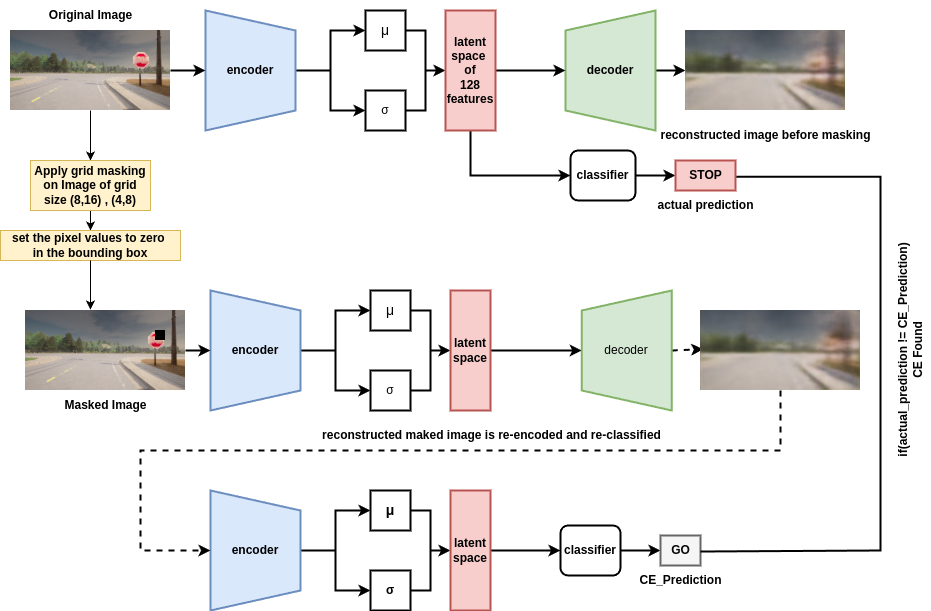
\includegraphics[width=0.95\textwidth]{img/masking/grid_based_masking/grid_based_masking_flow.drawio.png}
    \caption[Workflow of grid-based counterfactual generation]{Workflow of grid-based counterfactual generation. Grid cells are masked sequentially. If a prediction change occurs after VAE-based reconstruction, the masked region is considered causally influential.}
    \label{fig:grid_masking_diagram}
\end{figure}

Figure~\ref{fig:grid_ce_example} shows an example: an image originally classified as \texttt{STOP} changes to \texttt{GO} after masking a grid cell overlapping the STOP sign. This demonstrates that the masked region contained features that were critical for the classifier's decision. By reconstructing the masked image through the VAE, visual plausibility is preserved, ensuring that prediction changes are not caused by unrealistic artifacts.

\begin{figure}[htbp]
    \centering
    \begin{subfigure}[b]{0.3\textwidth}
        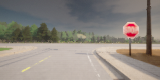
\includegraphics[width=\textwidth]{img/masking/grid_based_masking/original.png}
        \caption{Original Image}
        \label{fig:grid_orig}
    \end{subfigure}
    \hfill
    \begin{subfigure}[b]{0.3\textwidth}
        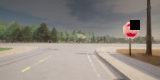
\includegraphics[width=\textwidth]{img/masking/grid_based_masking/reconstructed_grid_masked_image.png}
        \caption{Masked Grid Region}
        \label{fig:grid_masked}
    \end{subfigure}
    \hfill
    \begin{subfigure}[b]{0.3\textwidth}
        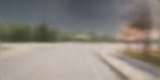
\includegraphics[width=\textwidth]{img/masking/grid_based_masking/CE_grid.png}
        \caption{Reconstructed CE Image}
        \label{fig:grid_recon}
    \end{subfigure}
    \caption[Grid-based counterfactual example]{Counterfactual example via grid-based masking. (a) Original image predicted as \texttt{STOP}. (b) Masking a cell over the STOP sign. (c) Reconstructed image predicted as \texttt{GO}, indicating the masked region's importance.}
    \label{fig:grid_ce_example}
\end{figure}


\clearpage

\subsection{Object Detection-Based Masking} \label{sec:object_detection_masking}

Object Detection-Based Masking introduces a semantically informed approach for generating counterfactual explanations by selectively removing identifiable real-world objects from complex driving scenes. The motivation behind this method is grounded in the causal interpretability of autonomous systems: understanding which specific entities—such as traffic signs, vehicles, pedestrians, or road infrastructure—directly influence a model's driving decision can provide actionable insights into the model's internal reasoning.

Following the general masking pipeline described in Section~\ref{sec:feature_masking_pipeline}, this approach utilizes a Variational Autoencoder (VAE) to encode the original input image into a latent space, which is then passed through a classifier to obtain the model’s initial prediction. However, rather than relying on low-level spatial patterns (as in grid-based masking), this method employs semantic object detection to guide the masking process.

To achieve this, a pre-trained YOLOv5 model~\cite{jocher2020yolov5} is integrated into the pipeline to detect and localize objects present in the input image. The full workflow is illustrated in Figure~\ref{fig:object_detection_workflow}, combining object detection, VAE-based reconstruction, and classifier re-evaluation to identify counterfactuals. YOLOv5 is a single-stage object detector known for its speed and accuracy across 80 COCO classes~\cite{lin2015microsoftcococommonobjects}, including vehicles, persons, and traffic control elements. Each detected object is described by a bounding box $(x_{\min}, y_{\min}, x_{\max}, y_{\max})$, which defines the region to be masked. The overall procedure is summarized in Algorithm~\ref{alg:object_detection_masking}.

\begin{figure}[htbp]
    \centering
    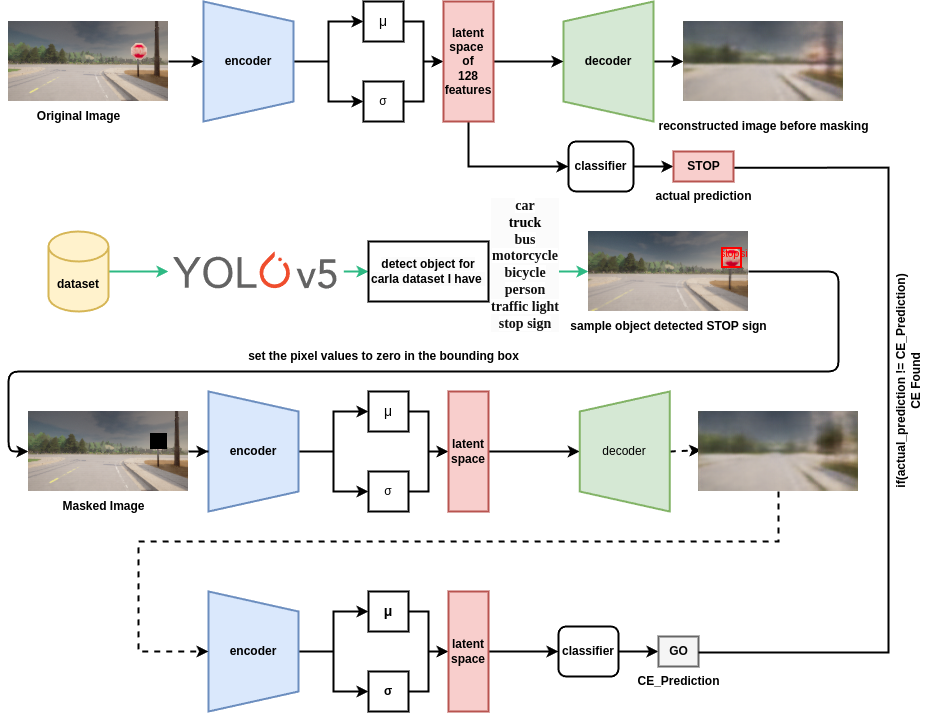
\includegraphics[width=0.95\textwidth]{img/masking/object_detection/object_detection_based_masking_flow.drawio.png}
    \caption[Workflow of object detection-based counterfactual generation]{%
    Workflow of the object detection-based counterfactual explanation pipeline. The input image is first encoded using a Variational Autoencoder (VAE) to obtain a latent representation. The classifier predicts the original driving decision (e.g., \texttt{STOP}). Simultaneously, a pre-trained YOLOv5 detector identifies objects in the image. One detected object (e.g., a STOP sign) is masked and passed through the encoder-decoder pipeline to reconstruct a visually plausible image. If reclassification of this reconstruction results in a different label (e.g., \texttt{GO}), a counterfactual explanation is found. The process is iterated per object, and the first valid counterfactual is retained.}
    \label{fig:object_detection_workflow}
\end{figure}

For each image, the process proceeds iteratively over all detected objects. The pixels inside the bounding box are zeroed out—effectively removing the object from the scene. This masked image is then processed through the VAE's encoder-decoder pipeline and re-classified. If the model's output label changes compared to the original prediction, a counterfactual explanation is said to have been generated. To adhere to the principle of minimal intervention~\cite{wachter2018CE}, only the first successful object level perturbation that triggers a label change is retained per image, ensuring a sparse and interpretable explanation.

In cases where multiple objects are detected but none cause the decision to flip, the method concludes that no object-level counterfactual exists for that specific scene. Additionally, if no objects are detected, the image is skipped from object-based masking consideration.

\vspace{1em}
\begin{algorithm}[h]
\caption{Object Detection-Based Masking for Counterfactual Generation}
\label{alg:object_detection_masking}
\begin{algorithmic}[1]
\REQUIRE Input image $I$, encoder $E$, decoder $D$, classifier $C$, object detector $Y$
\ENSURE Decision on whether a counterfactual explanation is found

\STATE Encode image: $z \leftarrow E(I)$
\STATE Predict original label: $y_{\text{orig}} \leftarrow \arg\max C(z)$
\STATE Detect objects using YOLO: $\mathcal{B} \leftarrow Y(I)$
\IF{$\mathcal{B}$ is empty}
    \RETURN No objects detected; no masking applied
\ENDIF
\FOR{bounding box $(x_{\min}, y_{\min}, x_{\max}, y_{\max}) \in \mathcal{B}$}
    \STATE Mask region in $I$ to obtain $I_{\text{masked}}$
    \STATE Encode: $z_{\text{masked}} \leftarrow E(I_{\text{masked}})$
    \STATE Decode: $I_{\text{recon}} \leftarrow D(z_{\text{masked}})$
    \STATE Re-encode: $z_{\text{re}} \leftarrow E(I_{\text{recon}})$
    \STATE Predict: $y_{\text{new}} \leftarrow \arg\max C(z_{\text{re}})$
    \IF{$y_{\text{new}} \neq y_{\text{orig}}$}
        \RETURN Counterfactual explanation found
    \ENDIF
\ENDFOR
\RETURN No counterfactual explanation found
\end{algorithmic}
\end{algorithm}
\vspace{1em}

This method brings semantic granularity to counterfactual explanation by connecting decisions with real-world entities, offering both interpretability and traceability. This is particularly valuable in autonomous driving, where decisions must often be justified not only in terms of performance but also in terms of safety-critical rationale.

\begin{figure}[htbp]
\centering
\begin{subfigure}[b]{0.24\textwidth}
    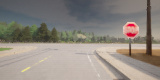
\includegraphics[width=\textwidth]{img/masking/object_detection/original.png}
    \caption{Original Image}
    \label{fig:orig}
\end{subfigure}
\hfill
\begin{subfigure}[b]{0.24\textwidth}
    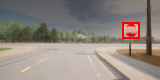
\includegraphics[width=\textwidth]{img/masking/object_detection/with_bbox.png}
    \caption{Object detected}
    \label{fig:orig_bbox}
\end{subfigure}
\hfill
\begin{subfigure}[b]{0.24\textwidth}
    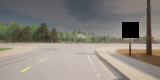
\includegraphics[width=\textwidth]{img/masking/object_detection/masked.png}
    \caption{Masked Image}
    \label{fig:masked}
\end{subfigure}
\hfill
\begin{subfigure}[b]{0.24\textwidth}
    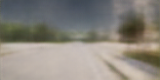
\includegraphics[width=\textwidth]{img/masking/object_detection/CE.png}
    \caption{Reconstructed Image}
    \label{fig:reconstructed}
\end{subfigure}
    \caption[Example of object detection-based counterfactual explanation]{%
    Counterfactual generation through object detection-based masking in a CARLA driving scene. (a) The original image as captured. (b) A STOP sign is detected and localized using YOLOv5. (c) The STOP sign is masked by zeroing out its bounding box. (d) The masked image is reconstructed using a Variational Autoencoder (VAE). The classifier changes its prediction from \texttt{STOP} to \texttt{GO}, indicating that the STOP sign was a causally decisive feature in the original decision.}
    \label{fig:object_detection_masking}
\end{figure}


Figure~\ref{fig:object_detection_masking} illustrates a concrete example of the object detection based masking process applied to a realistic driving scenario. The scene was rendered in the CARLA simulator and contains a STOP sign located on the right-hand side of the road.

The unaltered version of the image (Figure~\ref{fig:orig}) corresponds to the model's original input, for which the classifier predicts the label \texttt{STOP} with high confidence. The YOLOv5 object detector accurately identifies and localizes the STOP sign (Figure~\ref{fig:orig_bbox}), represented by a red bounding box. This is a safety-critical decision, expected in the presence of a regulatory traffic sign.

To probe the causal influence of the STOP sign, the region corresponding to the bounding box is zeroed out (Figure~\ref{fig:masked}). This masked image is then passed through a decoder which reconstructs the image in a smooth and naturalistic manner (Figure~\ref{fig:reconstructed}). The reconstruction effectively blurs or removes the masked STOP sign, preserving the surrounding context to remain within the data manifold.

Upon re-encoding and classifying the reconstructed image, the model changes its decision from \texttt{STOP} to \texttt{GO}. This prediction flip signifies a valid counterfactual explanation. The STOP sign was a critical feature in the model’s decision process. Its removal induced a behavioral shift, indicating a direct causal pathway between the visual presence of the STOP sign and the predicted driving action.

This example validates the semantic sensitivity of the proposed method. It reveals that object detection-based masking can expose model dependencies on interpretable, high-level visual cues, facilitating transparency in AI-driven navigation systems. The corresponding results on this method and comparing the effectiveness to other methods are detailed in \cref{sec:masking_eval}.





\subsection{LIME on Image-Based Masking}
\label{sec:lime_on_images}

Local Interpretable Model-Agnostic Explanations (LIME) is a post-hoc interpretability method that explains individual predictions by approximating a black-box model locally using an interpretable surrogate model~\cite{Ribeiro2018}. In the image domain, LIME operates by segmenting the input image into superpixels, selectively masking them, and observing the change in model predictions to determine which regions are most influential.

In this method, we integrate LIME into our counterfactual generation pipeline to test whether masking the most influential visual regions leads to a prediction flip. Specifically, we assess whether the top-$k$ superpixels (with $k=5$) identified by LIME as positively contributing to the predicted class are causally decisive. If masking these regions causes the classifier’s prediction to change, we consider this a successful counterfactual explanation (CE).

This method follows the unified pipeline described in Section~\ref{sec:feature_masking_pipeline}. The raw input image is first classified via a VAE-encoder and latent-space classifier setup. LIME is applied to the original image to compute the contribution of each superpixel to the classifier’s decision. Importantly, the prediction function passed to LIME encapsulates two steps: (i) encoding the perturbed image via the VAE encoder and (ii) computing class probabilities from the latent vector using the classifier.

For the masking step, we use a hard-masking strategy where the selected top-$k$ superpixels are set to zero (black). This choice aligns with the masking protocol used in grid-based and object detection-based methods, ensuring methodological consistency across techniques. The masking operation is defined as:
\[
I_{\text{masked}} = I \odot (1 - M),
\]
where \( I \) is the original image, and \( M \) is a binary mask indicating the superpixels selected by LIME.

After masking, the perturbed image is processed through the VAE’s encoder-decoder pathway to ensure reconstruction plausibility. The reconstructed image is re-encoded and reclassified. A change in classification outcome at this stage confirms the counterfactual nature of the masked regions.

The full workflow is illustrated in Figure~\ref{fig:lime_image_workflow}, and the algorithmic steps are formalized in Algorithm~\ref{alg:lime_on_images}. This visual pipeline emphasizes the sequential transformation from original input to counterfactual outcome, highlighting LIME’s role in superpixel selection and the VAE’s function in generating visually coherent explanations.

\begin{figure}[htbp]
    \centering
    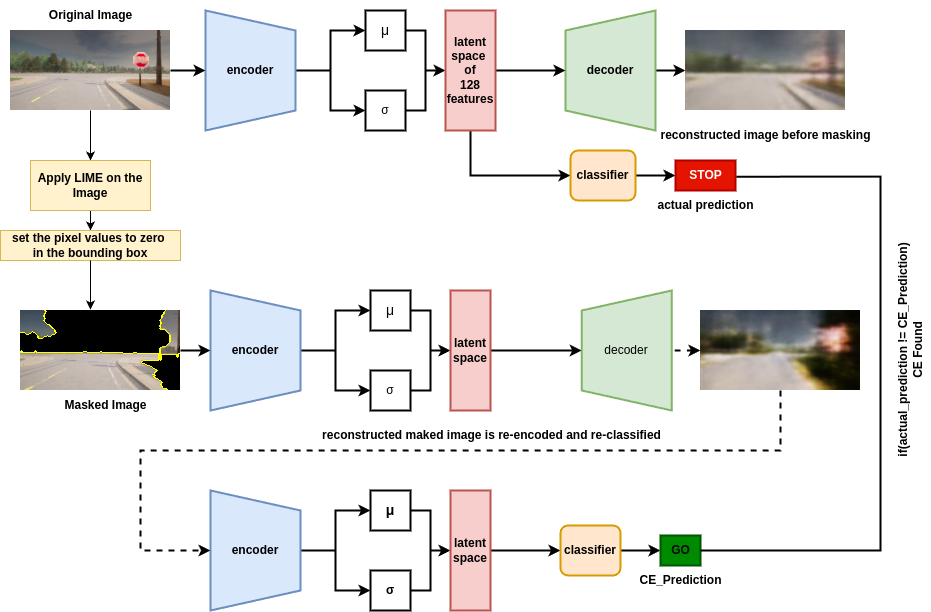
\includegraphics[width=0.95\textwidth]{img/masking/lime_on_images/lime_on_images_based_masking_flow.drawio.png}
    \caption[Workflow of LIME-based counterfactual generation]{%
Workflow of the LIME-based counterfactual explanation pipeline. The input image is classified through the VAE encoder and classifier. LIME identifies top-$k$ superpixels, which are hard-masked. The masked image is reconstructed via the decoder, re-encoded, and reclassified. A prediction flip indicates a successful counterfactual explanation.}
    \label{fig:lime_image_workflow}
\end{figure}



\begin{algorithm}[htbp]
\caption{LIME on Images for Counterfactual Generation (Hard Masking)}
\label{alg:lime_on_images}
\begin{algorithmic}[1]
\REQUIRE Image $I$, encoder $E$, decoder $D$, classifier $C$, LIME explainer $L$
\ENSURE Whether a counterfactual explanation is found

\STATE $z \leftarrow E(I)$ \hfill // Encode original image
\STATE $y_{\text{orig}} \leftarrow \arg\max C(z)$ \hfill // Predict original class
\STATE $M \leftarrow L(I, C)$ \hfill // Compute LIME mask
\STATE $R \leftarrow \text{Mask}(M, k=5)$ \hfill // Select top-$k$ superpixels
\STATE $I_{\text{masked}} \leftarrow I \odot (1 - R)$ \hfill // Apply hard masking
\STATE $z_{\text{masked}} \leftarrow E(I_{\text{masked}})$
\STATE $I_{\text{recon}} \leftarrow D(z_{\text{masked}})$
\STATE $z_{\text{re}} \leftarrow E(I_{\text{recon}})$
\STATE $y_{\text{new}} \leftarrow \arg\max C(z_{\text{re}})$
\IF{$y_{\text{new}} \neq y_{\text{orig}}$}
    \RETURN Counterfactual explanation found
\ENDIF
\RETURN No counterfactual explanation found
\end{algorithmic}
\end{algorithm}

\begin{figure}[htbp]
\centering
\begin{subfigure}[b]{0.3\textwidth}
    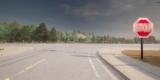
\includegraphics[width=\textwidth]{img/appendix/original_town7_000980.png}
    \caption{Original Image (\texttt{STOP})}
    \label{fig:lime_orig}
\end{subfigure}
\hfill
\begin{subfigure}[b]{0.3\textwidth}
    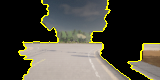
\includegraphics[width=\textwidth]{img/appendix/LIME_on_Image_maksed_town7_000980.png}
    \caption{LIME-masked Superpixels}
    \label{fig:lime_masked}
\end{subfigure}
\hfill
\begin{subfigure}[b]{0.3\textwidth}
    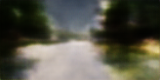
\includegraphics[width=\textwidth]{img/appendix/LIME_on_Image_reconstructed_town7_000980.png}
    \caption{Reconstructed Image (\texttt{GO})}
    \label{fig:lime_recon}
\end{subfigure}
\caption[Example of counterfactual via LIME on images]{%
Example of counterfactual explanation using LIME-based image masking. (a) The original input is classified as \texttt{STOP}. (b) Top-5 superpixels identified by LIME are masked. (c) The reconstructed image causes the model to flip its prediction to \texttt{GO}, indicating those regions were causally decisive.}
\label{fig:lime_image_example}
\end{figure}




Figure~\ref{fig:lime_image_example} illustrates a concrete example where masking the LIME-identified regions causes the prediction to flip from \texttt{STOP} to \texttt{GO}, indicating the effectiveness of the selected superpixels in driving the original decision.



Compared to grid-based or object detection-based masking, LIME provides an adaptive, model-agnostic strategy for identifying causally important regions. Unlike fixed spatial masking, it focuses only on the most relevant superpixels for a specific prediction. The comparative evaluation of this method is presented in Section~\ref{sec:masking_eval}.





\clearpage
% \vspace{1em}
\subsection{LIME-Based Masking on Latent Features} \label{sec:lime_based_masking_on_latent_features}

\subsubsection*{Latent Feature Statistics Preprocessing}
\label{sec:latent_statistics_preprocessing}

Before applying LIME in the latent space, we compute dataset-level priors to ensure plausible latent perturbations. All images from the dataset are passed through the trained Variational Autoencoder (VAE) encoder to extract their 128-dimensional latent representations. From these, per-dimension statistics such as mean, median, min, max, and standard deviation are calculated. These values are stored and later used to replace influential latent features with neutral values (e.g., medians), helping to preserve semantic coherence during counterfactual generation.




\subsection{LIME on Latent Features Masking}
\label{sec:lime_on_latent}

In this approach, LIME is applied directly to the VAE latent space to identify and perturb the most influential latent dimensions responsible for a classifier’s decision. Unlike its image-space counterpart, this method enables counterfactual reasoning at a higher semantic level.

As illustrated in Figure~\ref{fig:lime_latent_workflow}, the input image \( I \) is encoded into a latent vector \( z = E(I) \), and a downstream classifier \( C \) predicts the class \( y_{\text{orig}} = \arg\max C(z) \). LIME is then applied to this latent vector using a prediction function composed of \( C \circ E \), producing a ranked list of feature importances \( \{(w_i, i)\} \), where \( w_i \) is the importance of latent dimension \( i \).

Only positively contributing features (i.e., \( w_i > 0 \)) are considered for masking. These are sorted in descending order of influence to form the set \( \mathcal{F} = \{i_1, i_2, \ldots, i_k\} \). For each index \( i \in \mathcal{F} \), we iteratively replace \( z_i \) with its corresponding median \( \bar{z}_i \) from the dataset:

\[
z_i^{\text{masked}} =
\begin{cases}
\bar{z}_i & \text{if } i \in \mathcal{F}_{\text{used}} \\
z_i & \text{otherwise}
\end{cases}
\]

The modified latent vector is decoded into an image \( I_{\text{recon}} = D(z^{\text{masked}}) \), re-encoded, and re-classified. If the predicted label \( y_{\text{new}} = \arg\max C(E(I_{\text{recon}})) \) differs from the original prediction, a counterfactual explanation is found.

Figure~\ref{fig:lime_latent_example} shows a qualitative example, including the original image, LIME importance plot, masked latent dimensions, and the reconstructed counterfactual. The red bars in the importance plot indicate features contributing to the original class (\texttt{STOP}), and the green bars indicate opposing contributions. The classifier prediction flips to \texttt{RIGHT} after masking 12 latent features, illustrating the causal role of these high-level representations.

\vspace{0.5em}
\begin{figure}[h]
\centering
    \begin{subfigure}{0.24\textwidth}
        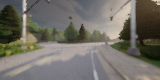
\includegraphics[width=\linewidth]{img/masking/lime_on_latent/original.png}
        \caption*{(a) Original image}
    \end{subfigure}
    \hfill
    \begin{subfigure}{0.72\textwidth}
        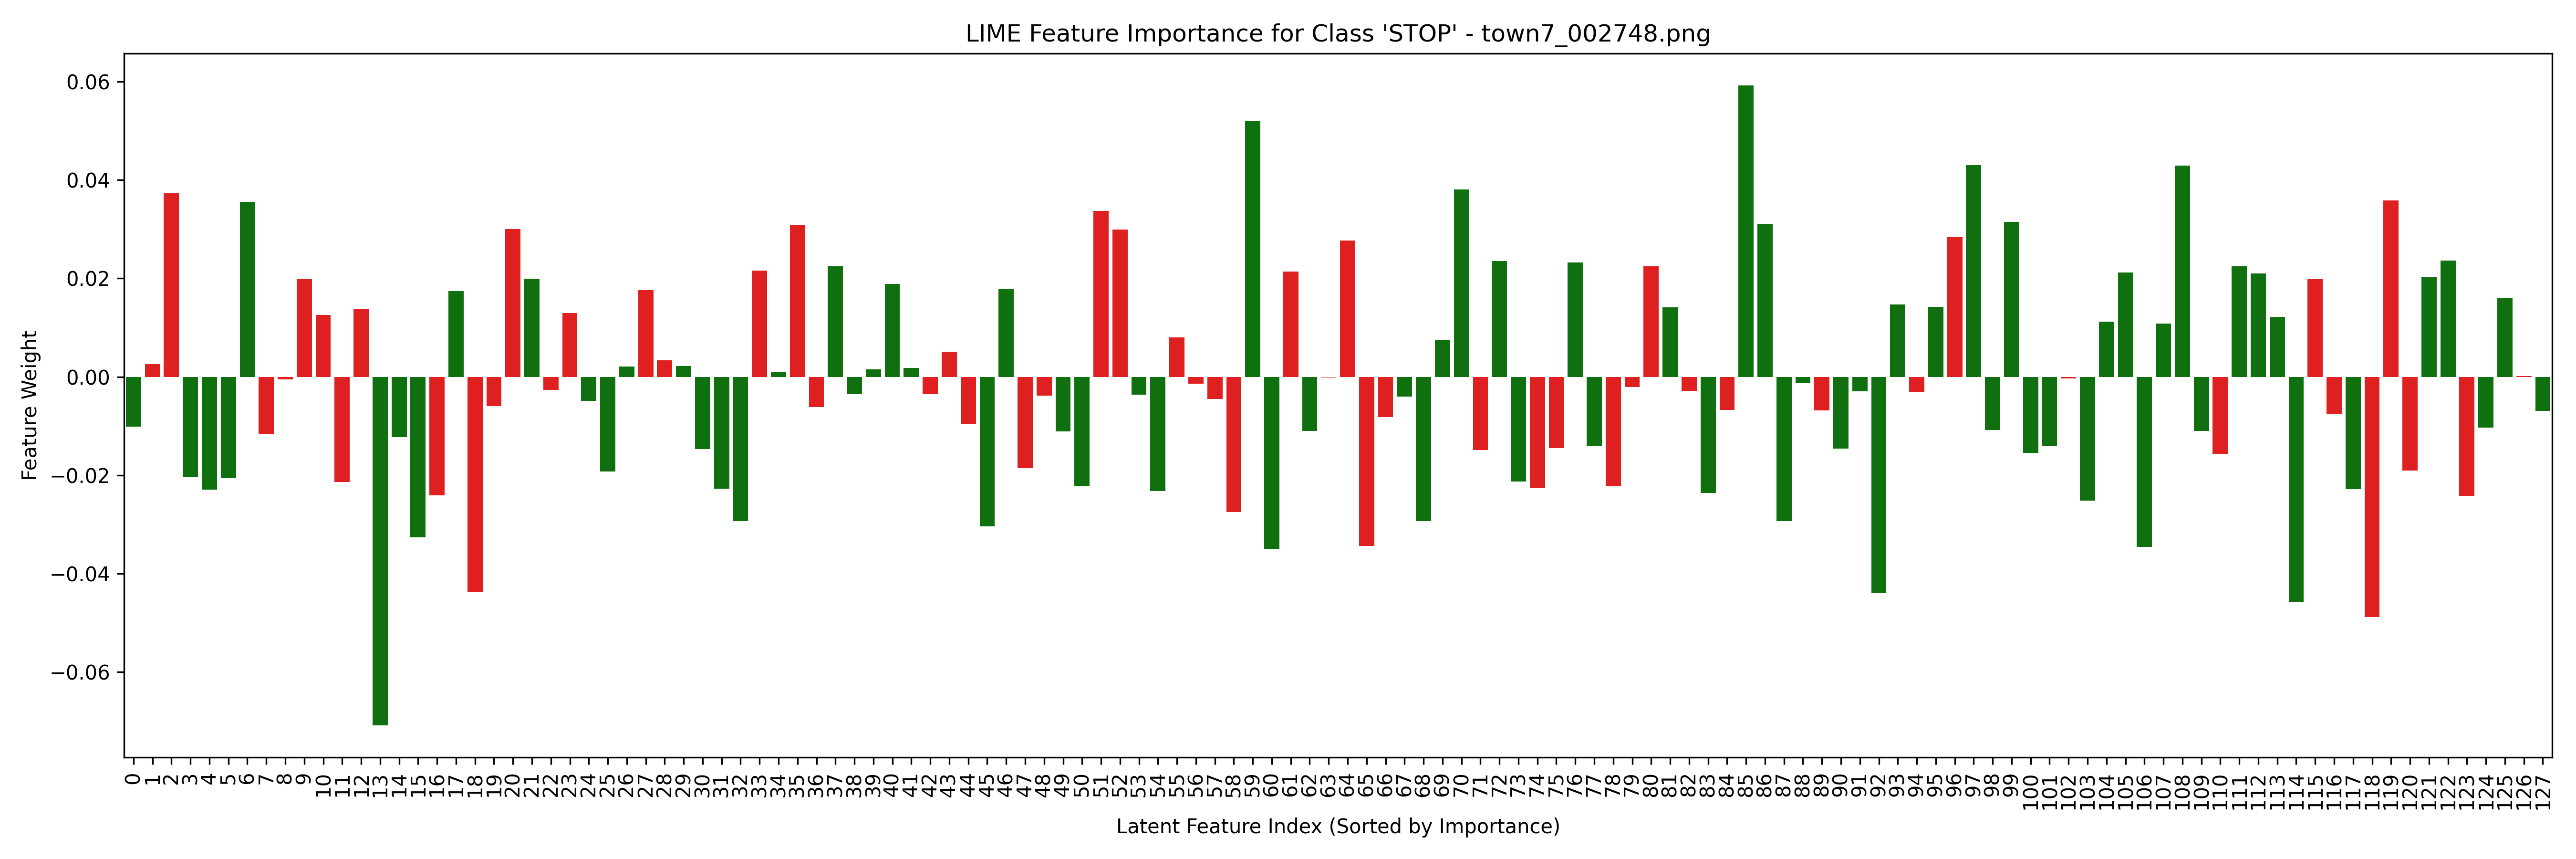
\includegraphics[width=\linewidth]{img/masking/lime_on_latent/town7_002748.png_lime_feature_importance_class_STOP_sorted.png}
        \caption*{(b) LIME importance plot for class \texttt{STOP}}
    \end{subfigure}
    
    \vspace{0.5em}
    
    \begin{subfigure}{0.72\textwidth}
        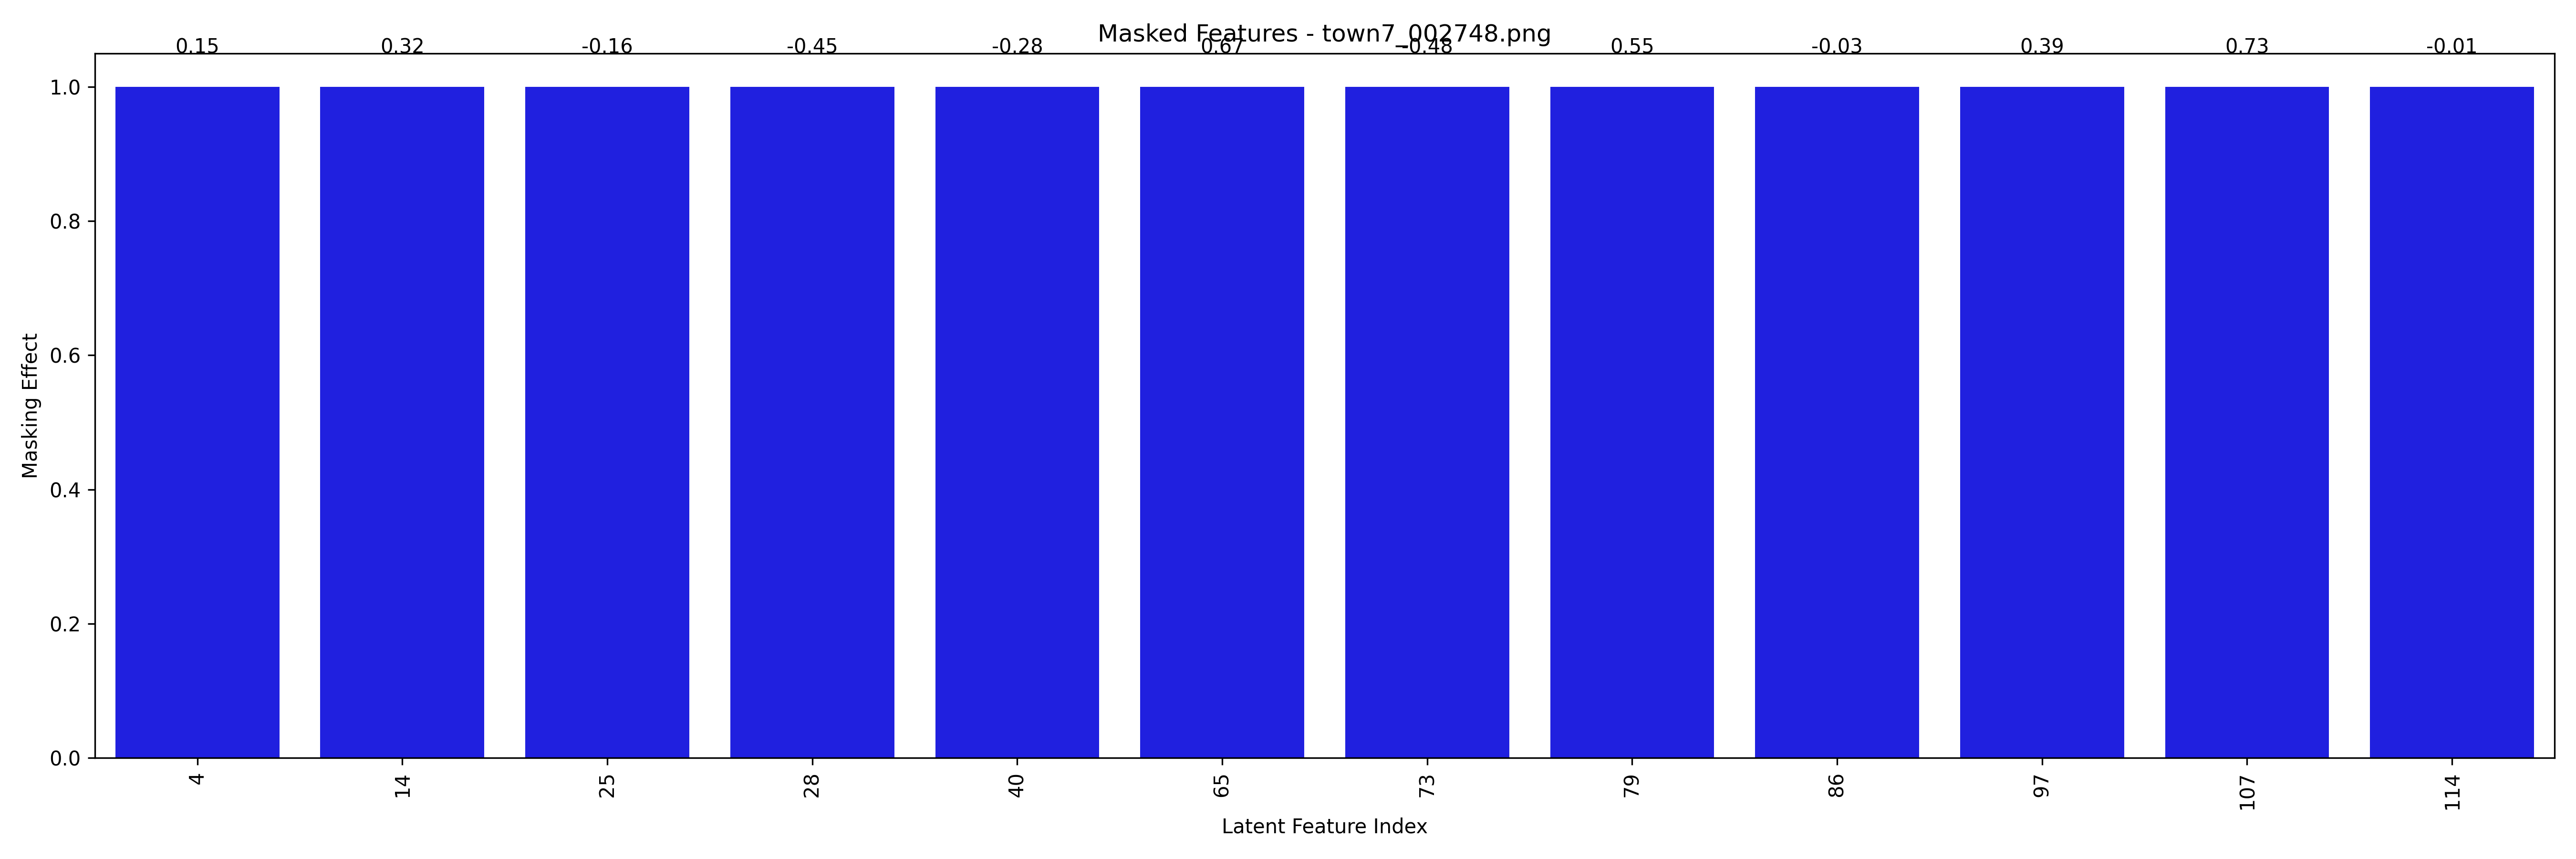
\includegraphics[width=\linewidth]{img/masking/lime_on_latent/town7_002748.png_masked_features.png}
        \caption*{(c) Masked features with their weights}
    \end{subfigure}
    \hfill
    \begin{subfigure}{0.24\textwidth}
        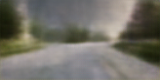
\includegraphics[width=\linewidth]{img/masking/lime_on_latent/reconstructed_lime_on_features.png}
        \caption*{(d) Reconstructed counterfactual}
    \end{subfigure}

    \caption[Example of LIME-based latent feature masking]{%
LIME on latent space masking. The input image was originally classified as \texttt{STOP} (confidence: 52.5\%). LIME identified the most influential latent features, which were replaced with their corresponding median values. After masking 12 features, the prediction flipped to \texttt{RIGHT} (confidence: 48.3\%).}
    \label{fig:lime_latent_example}
\end{figure}

\begin{figure}[h]
    \centering
    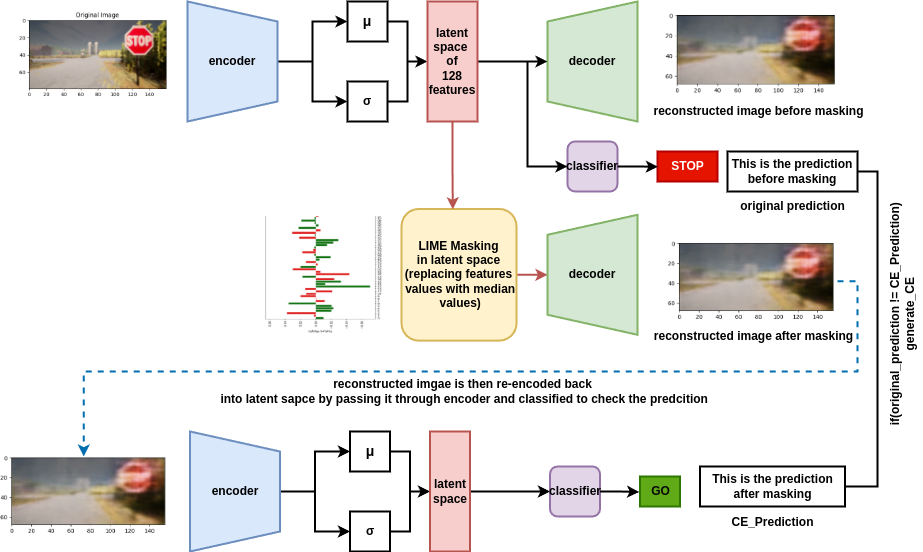
\includegraphics[width=0.95\linewidth]{img//masking/lime_on_latent/LIME_on_latent_space_masking.png}
    \caption[Workflow of LIME-based latent feature masking]{%
Workflow of LIME-based latent space masking. After VAE encoding and classification, positively contributing latent features (as identified by LIME) are replaced with dataset-level median values. The decoder reconstructs a perturbed image, which is then re-encoded and re-classified. A prediction change indicates a successful counterfactual.}
    \label{fig:lime_latent_workflow}
\end{figure}

The full procedure is detailed in Algorithm~\ref{alg:lime_on_latent}, which describes how influential latent features are selected, masked using dataset-informed statistics, and evaluated to determine counterfactual validity.

\vspace{0.5em}
\begin{algorithm}[h]
\caption{LIME-Based Masking on Latent Features}
\label{alg:lime_on_latent}
\begin{algorithmic}[1]
\REQUIRE Image $I$, encoder $E$, decoder $D$, classifier $C$, median latent vector $\bar{z}$
\ENSURE Whether a counterfactual explanation is found

\STATE $z \leftarrow E(I)$ \hfill // Encode to latent vector
\STATE $y_{\text{orig}} \leftarrow \arg\max C(z)$
\STATE Compute LIME explanations on $z$ w.r.t.\ $C$
\STATE Select top positively contributing features \( \mathcal{F} \)
\FOR{each $i \in \mathcal{F}$}
    \STATE Replace $z_i \leftarrow \bar{z}_i$
    \STATE $I_{\text{recon}} \leftarrow D(z)$
    \STATE $z_{\text{re}} \leftarrow E(I_{\text{recon}})$
    \STATE $y_{\text{new}} \leftarrow \arg\max C(z_{\text{re}})$
    \IF{$y_{\text{new}} \ne y_{\text{orig}}$}
        \RETURN Counterfactual explanation found
    \ENDIF
\ENDFOR
\RETURN No counterfactual explanation found
\end{algorithmic}
\end{algorithm}

This method offers a conceptually powerful framework for counterfactual generation. By perturbing high-level latent features instead of raw pixels, it ensures more interpretable and semantically grounded explanations. The use of statistical priors and early stopping improves both plausibility and computational efficiency. Comparative results and metrics for this method are discussed in Section~\ref{sec:masking_eval}.



\clearpage

\subsection{LIME-Guided Latent Feature Masking using NUN} \label{lime_with_NUN}

In this work, we extend the counterfactual explanation strategy introduced by Wijekoon et al.~\cite{WijekoonWNMPC21} to the domain of deep generative models. While originally applied to tabular data, we adapt their approach to the latent space of image representations learned by a Variational Autoencoder (VAE) which is again a tabular data. Specifically, we implement Method 2, in which LIME a post-hoc method is applied to the latent vector of a \textit{Nearest Unlike Neighbor} (NUN)~\cite{DELANEY2023103995} to guide feature replacement in the query representation until a class change is achieved.

Given an input image \( x \), we encode it into a latent vector \( z \) using a pretrained VAE encoder \( E \), and obtain its predicted class \( y = \arg\max C(z) \) from a trained classifier \( C \). We then identify the Nearest Unlike Neighbor \( \hat{z} \), which belongs to a different predicted class \( \hat{y} \ne y \), by computing the Euclidean distance in the latent space:

\[
\hat{z} = \arg\min_{z_j \in \mathcal{D}_{\text{test}}} \left\{ \| z - z_j \|_2 \; \middle| \; C(z_j) \ne y \right\}
\]

This NUN latent vector represents a semantically similar example that yields a different classification, and thus serves as a candidate for counterfactual explanation generation.

\begin{figure}[h]
    \centering
    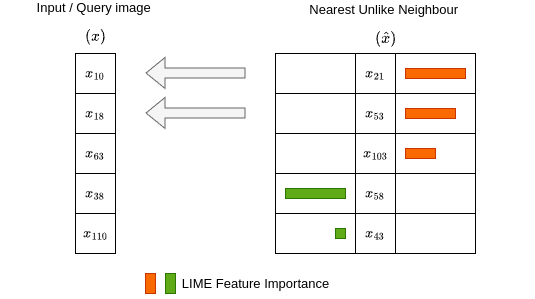
\includegraphics[width=0.55\textwidth]{img/masking/lime_on_latent_nun/NUN_method.drawio.png}
    \caption[Concept of LIME with NUN feature transfer]{%
Illustration of the proposed method. Important latent features (as determined by LIME) are transferred from the NUN to the input in order of decreasing importance until the classifier's prediction changes.}
    \label{fig:nun_lime_concept}
\end{figure}

To prioritize the most relevant feature changes, we apply the \textit{LIME Tabular Explainer}~\cite{Ribeiro2018} to the NUN vector \( \hat{z} \). LIME generates a local surrogate model that assigns importance weights to each latent feature, resulting in an ordered list:

\[
\text{AFOrderLIME}(\hat{z}) = \{ i_1, i_2, \dots, i_m \}, \quad \text{where } |w_{i_1}| > |w_{i_2}| > \dots > |w_{i_m}|
\]

These weights reflect how much each latent feature contributes to the predicted class of the NUN. We use this ranking to iteratively transfer features from \( \hat{z} \) to the query vector that is input image vector\( z \).

\begin{figure}[h]
    \centering
    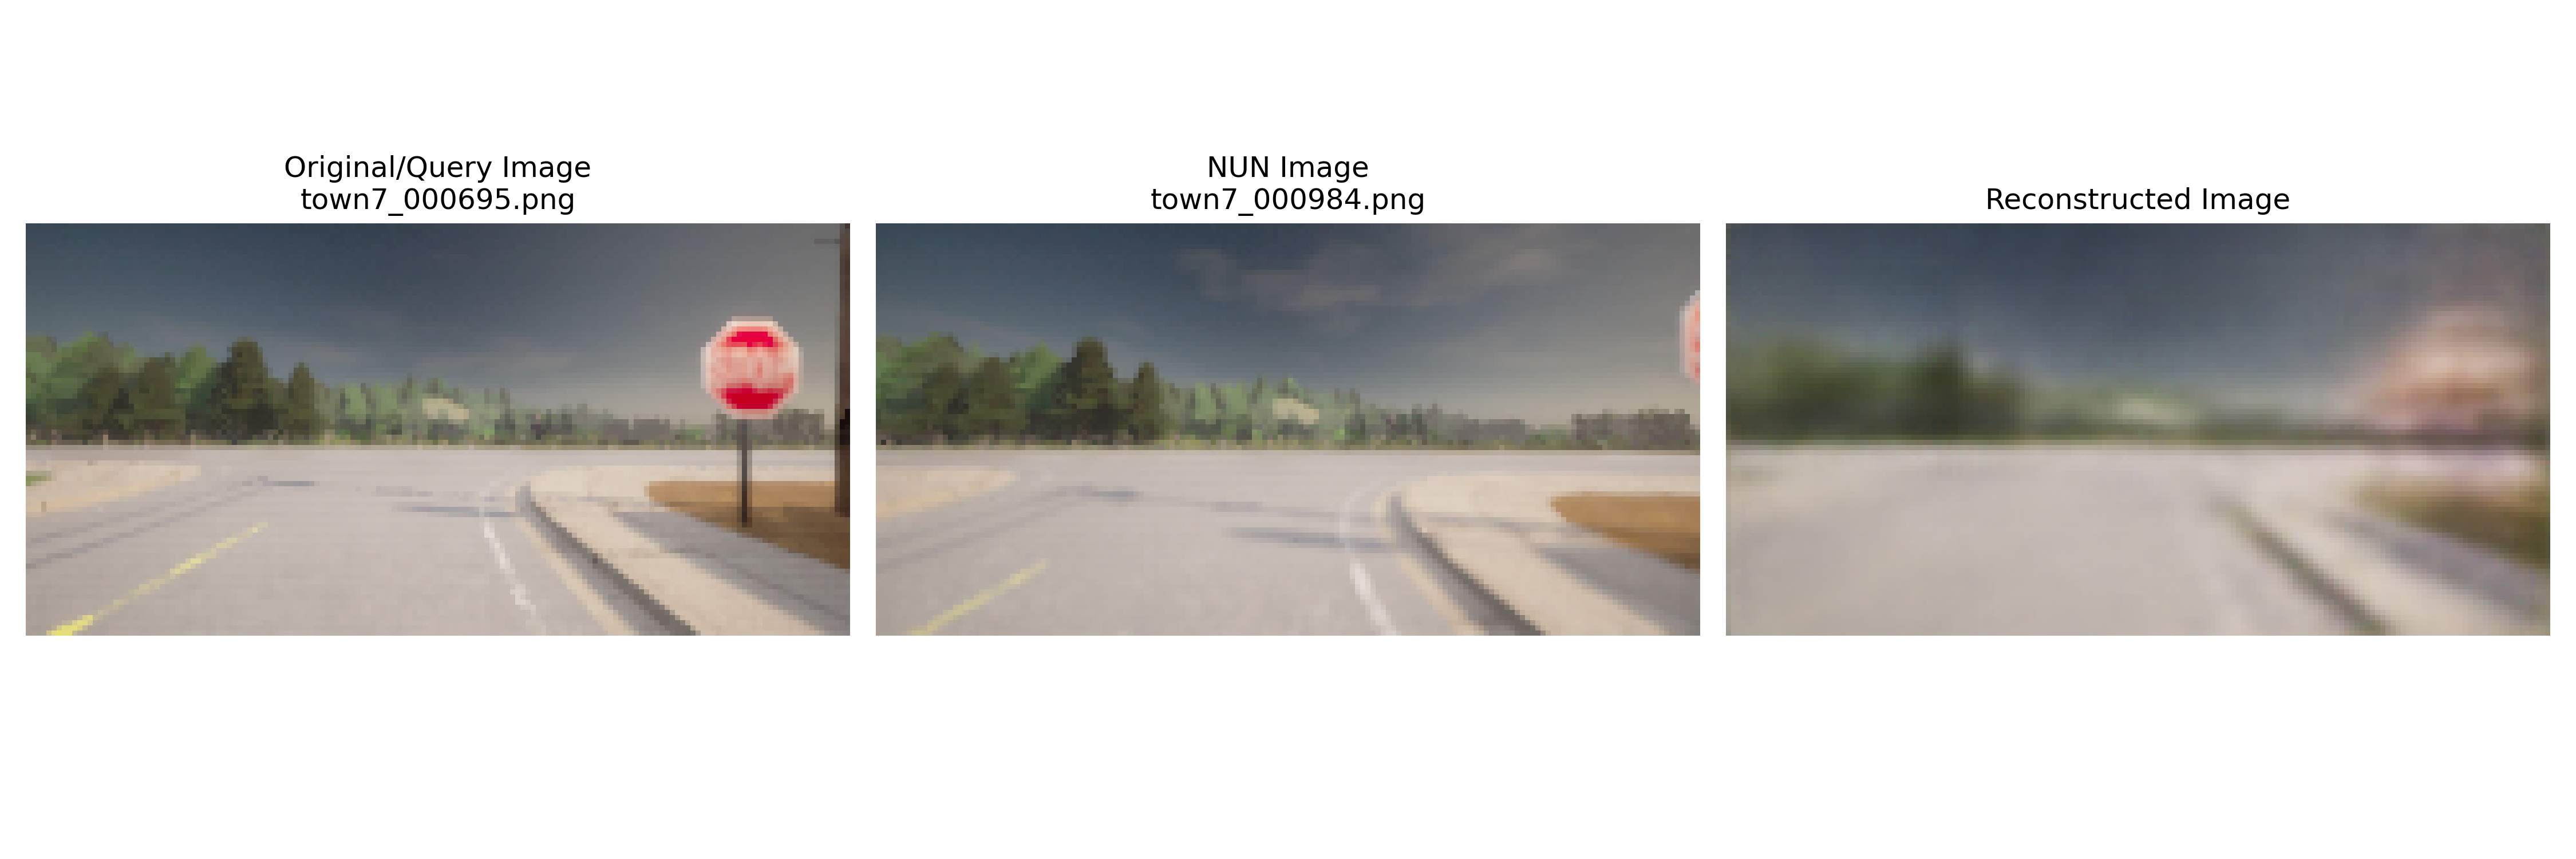
\includegraphics[width=\linewidth]{img//masking//lime_on_latent_nun/town7_000695.png_side_by_side.png}
    \caption[Example of LIME-NUN counterfactual generation]{%
Visual comparison of LIME-guided latent feature masking using Nearest Unlike Neighbor (NUN). 
Left: Query image originally classified as \texttt{STOP}. 
Middle: Its nearest unlike neighbor classified as \texttt{GO}. 
Right: Reconstructed counterfactual image where the prediction flips to \texttt{GO}.}
    \label{fig:nun_cf_side_by_side}
\end{figure}


Following the LIME importance order, each dimension is replaced via \( z[i_k] \leftarrow \hat{z}[i_k] \), and the modified latent vector \( z' \) is reconstructed into an image \( x' = D(z') \). The reconstructed image is re-encoded and re-classified to determine whether a class change has occurred. This process continues until the prediction flips, identifying a minimal set of latent features required to finding a counterfactual explanation. The complete procedure is summarized in Algorithm~\ref{alg:nun_lime} and the workflow is is shown in Figure~\ref{fig:nun_lime_workflow}



\begin{figure}[h]
    \centering
    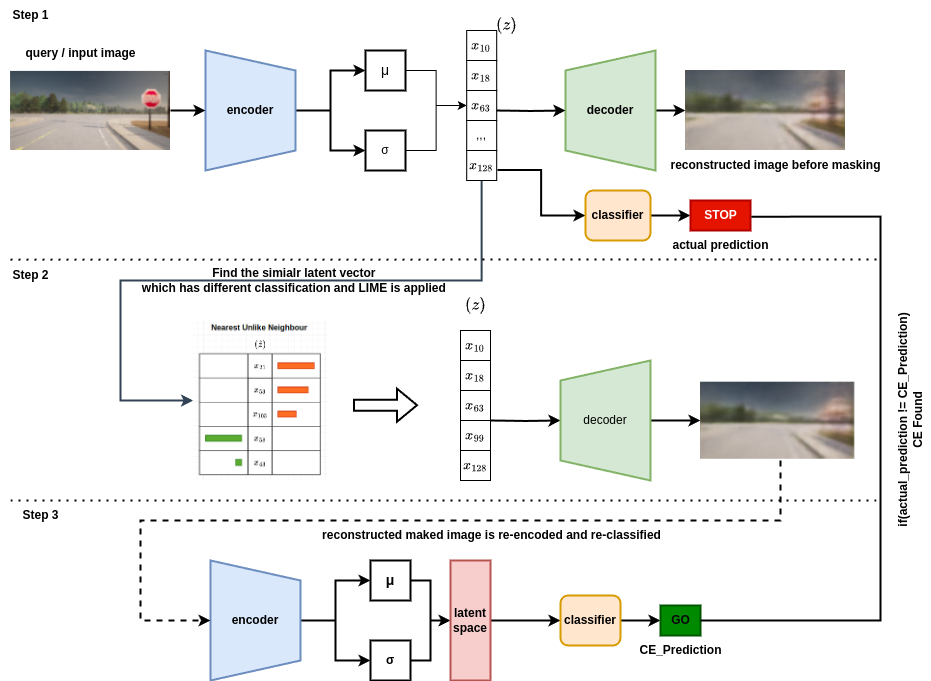
\includegraphics[width=0.95\textwidth]{img/masking/lime_on_latent_nun/lime_on_latent_featuring_using_NUN.png}
    \caption[Workflow of LIME-guided latent masking with NUN]{%
Workflow of the LIME-Guided Latent Feature Masking using Nearest Unlike Neighbor (NUN).  
Step 1: The query image is encoded into a 128-dimensional latent vector using the VAE encoder and classified to obtain the original prediction (\texttt{STOP}).  
Step 2: A latent vector from the test set with a different class prediction (NUN) is selected based on Euclidean proximity. LIME is applied to the NUN to rank the most influential latent features. These top-$k$ features are iteratively transferred from the NUN to the query latent vector.  
Step 3: After each replacement, the vector is decoded, re-encoded, and re-classified. If the prediction changes (e.g., to \texttt{GO}), the change is recorded as a counterfactual explanation.}
    \label{fig:nun_lime_workflow}
\end{figure}




An illustration of this feature transfer mechanism is shown in Figure~\ref{fig:nun_lime_concept}. The left column depicts the latent features of the input image, while the right column represents the features of its NUN. LIME-assigned importance is indicated through color-coded bars. Features with higher importance are prioritized during transfer from the NUN to the query. Arrows between the two vectors highlight the flow of values during the masking process.


\begin{algorithm}[h]
\caption{LIME-Based Masking on Latent Features using NUN}
\label{alg:nun_lime}
\begin{algorithmic}[1]
\REQUIRE Encoder $E$, Decoder $D$, Classifier $C$, Query image $I$, Test dataset $\mathcal{D}_{\text{test}}$, Label mapping $\mathcal{L}$
\ENSURE Counterfactual image $x_{\text{cf}}$, Number of features replaced $k$, Evaluation metrics

\STATE $z \leftarrow E(I)$ \hfill \textit{// Encode query to latent space}
\STATE $y \leftarrow \arg\max C(z)$ \hfill \textit{// Get predicted label}
\STATE $z_{\text{NUN}} \leftarrow \text{None}$, $d_{\min} \leftarrow \infty$

\FORALL{$J \in \mathcal{D}_{\text{test}}$}
    \STATE $z_j \leftarrow E(J)$
    \STATE $y_j \leftarrow \arg\max C(z_j)$
    \IF{$y_j \ne y$}
        \STATE $d \leftarrow \|z - z_j\|_2$
        \IF{$d < d_{\min}$}
            \STATE $z_{\text{NUN}} \leftarrow z_j$
            \STATE $d_{\min} \leftarrow d$
        \ENDIF
    \ENDIF
\ENDFOR

\STATE $importance \leftarrow \text{LIME}(\hat{z}, C)$ \hfill \textit{// Explain NUN's classification}
\STATE $\mathcal{F} \leftarrow \text{AFOrderLIME}(\hat{z})$ \hfill \textit{// Sort features by decreasing $|w_i|$}
\STATE $z_{\text{mod}} \leftarrow z$, $k \leftarrow 0$

\FORALL{$i \in \mathcal{F}$}
    \STATE $z_{\text{mod}}[i] \leftarrow z_{\text{NUN}}[i]$
    \STATE $x_{\text{recon}} \leftarrow D(z_{\text{mod}})$
    \STATE $z_{\text{reenc}} \leftarrow E(x_{\text{recon}})$
    \STATE $y_{\text{new}} \leftarrow \arg\max C(z_{\text{reenc}})$
    \STATE $k \leftarrow k + 1$
    \IF{$y_{\text{new}} \ne y$}
        \STATE \textbf{break}
    \ENDIF
\ENDFOR

\STATE $\text{metrics} \leftarrow \text{Evaluate}(I, x_{\text{recon}})$
\RETURN $x_{\text{recon}}, k, \text{metrics}$
\end{algorithmic}
\end{algorithm}


This approach leverages LIME’s interpretability and the semantic richness of the latent space to generate actionable counterfactuals. It ensures minimal intervention while maintaining high visual fidelity, and directly aligns with the counterfactual generation principles outlined by Wijekoon et al.~\cite{WijekoonWNMPC21}. The corresponding results on this method and comparing the effectiveness to other methods are detailed in \cref{sec:masking_eval}.